%20 min preso!
\documentclass[xcolor=table,english]{beamer}
\usepackage{beamerthemesplit}
\usepackage{wrapfig}
\usetheme{SPbGU}
\usepackage{pdfpages}
\usepackage{amsmath}
\usepackage{mathtools}
\usepackage{cmap}
\usepackage{subcaption}
\usepackage[utf8]{inputenc}
\usepackage[T1, T2A]{fontenc}
\usepackage[]{babel}
\usepackage{indentfirst}
\usepackage{amsmath}
\usepackage{tikz}
\usepackage{multirow}
\usepackage[noend]{algpseudocode}
\usepackage{algorithm}
\usepackage{algorithmicx}
\usepackage{fancyvrb}
\usetikzlibrary{calc}
\usetikzlibrary{shapes,arrows}
\usetikzlibrary{arrows,automata}
\usetikzlibrary{positioning}
\usetikzlibrary{fit}

\usepackage{kbordermatrix} % include package @ document preamble
\renewcommand{\kbldelim}{(} % change default array delimiters to parentheses
\renewcommand{\kbrdelim}{)}

\newcommand\mca{\multicolumn{1}{c}{\cellcolor{red}\textbf{\{a\}}}}
\newcommand\mcb{\multicolumn{1}{c}{\cellcolor{red}\textbf{\{b\}}}}

\usepackage{tabularx}
\newcolumntype{Y}{>{\raggedleft\arraybackslash}X}

\renewcommand{\thealgorithm}{}

\newtheorem{mytheorem}{Theorem}
\renewcommand{\thealgorithm}{}

\newcommand{\tikzmark}[1]{\tikz[overlay,remember picture] \node (#1) {};}
\def\Put(#1,#2)#3{\leavevmode\makebox(0,0){\put(#1,#2){#3}}}

\newcommand{\ltz}{$< 1$}


\tikzset{
    state/.style={
           rectangle,
           rounded corners,
           draw=black, very thick,
           minimum height=2em,
           inner sep=2pt,
           text centered,
           },
}

\beamertemplatenavigationsymbolsempty

\title[Graphs Traveral GPU]{Efficient Memory-access for Out-of-memory Graph-traversal In GPUs}
% \subtitle[YaccConstructor]{Parsing techniques for graph analysis}
% То, что в квадратных скобках, отображается в левом нижнем углу.
\institute[СПбГУ]{
JetBrains Research, Лаборатория языковых инструментов  \\
Санкт-Петербургский Государственный университет
}

% То, что в квадратных скобках, отображается в левом нижнем углу (прикольно).
\author[Егор Орачев]{\textbf{Егор Орачев}}
\date{20 октября 2020}


\begin{document}
{
\begin{frame}[fragile]
  \begin{table}
  \centering
  \begin{tabularx}{\linewidth}{YcX}
    
\includegraphics[height=1.5cm]{pictures/jetbrainsResearch.pdf} \hfill
    & \begin{minipage}[t]{0.3\textwidth}\center \vspace{-1cm}  Семинар
      \end{minipage}
    & \hfill 
\includegraphics[height=1.5cm]{pictures/SPbGU_Logo.png}
  \end{tabularx}
  \end{table}
  \titlepage
\end{frame}
}

\begin{frame}[fragile] \frametitle{Мотивация} 
    \begin{minipage}[m]{0.45\linewidth}
        \begin{figure}
            \centering
            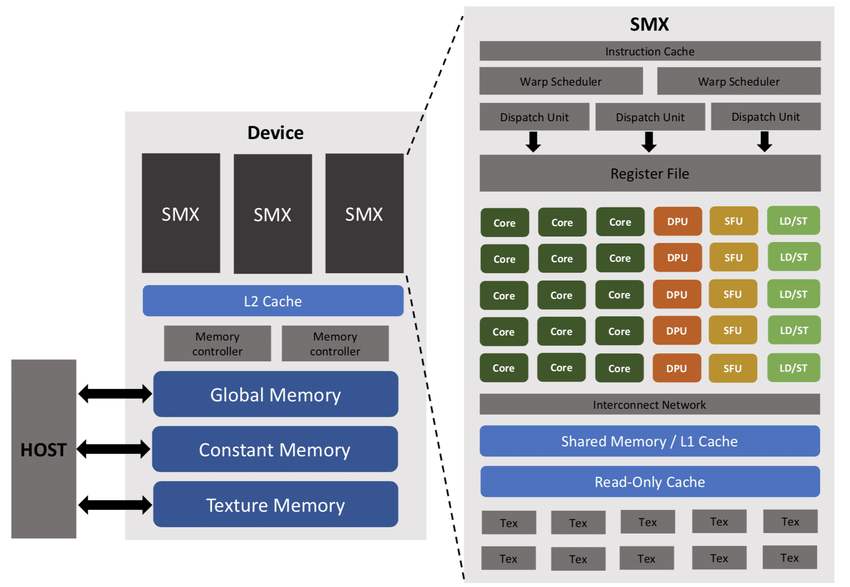
\includegraphics[width=\textwidth]{pictures/gpu_architecture.png}
            \caption{Generic GPU Architecture}
            \label{fig:architecture}
        \end{figure}
    \end{minipage}\hfill
    \begin{minipage}[m]{0.55\linewidth}
        \begin{itemize}
            \item Современные системы аналитики и рекомендаций все чаще строятся на основе     анализа графовых данных
            \item Реальные графовые данные имеют невероятно большой размер
            \item Возможность для распараллеливания обработки
            \item Использование GPU для решения подобного рода задач
        \end{itemize}
    \end{minipage}
\end{frame}

\begin{frame}[fragile] \frametitle{Взгляд с высоты}
    \begin{center}
    \begin{minipage}[m]{0.8\linewidth}
        \begin{figure}
            \centering
            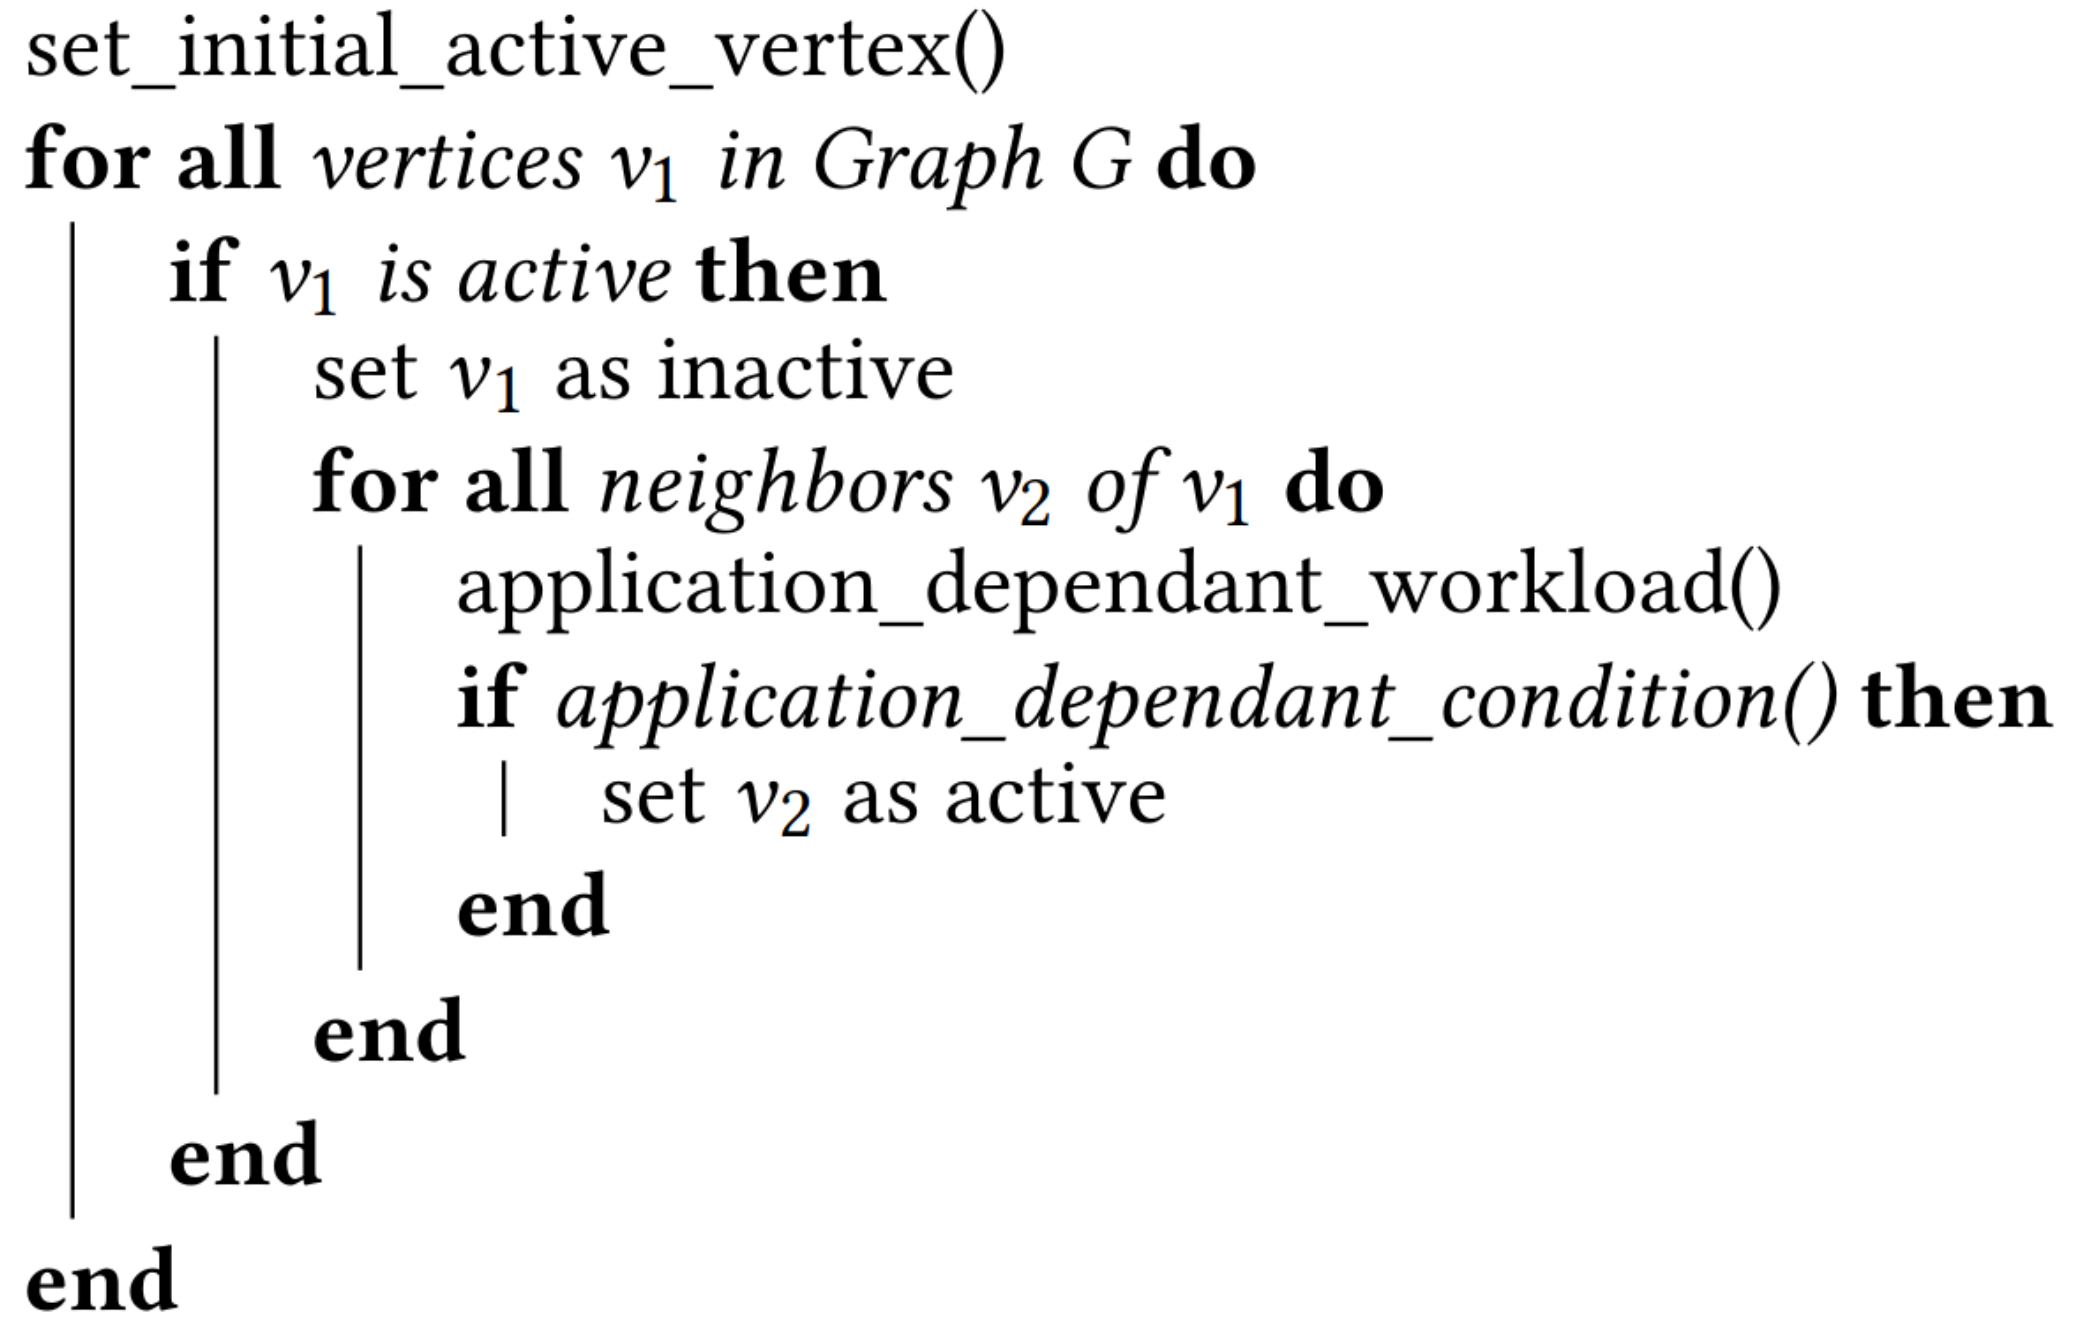
\includegraphics[width=\textwidth]{figures/high_level_algo.png}
            \caption{High-level graph traversal flow}
            \label{fig:high_level_algo}
        \end{figure}
    \end{minipage}\hfill
    \end{center}
\end{frame}

\begin{frame}[fragile] \frametitle{Пример графа и матрицы}
    \begin{minipage}[m]{1.0\linewidth}
        \begin{figure}
            \centering
            \begin{subfigure}[b]{0.47\textwidth}
                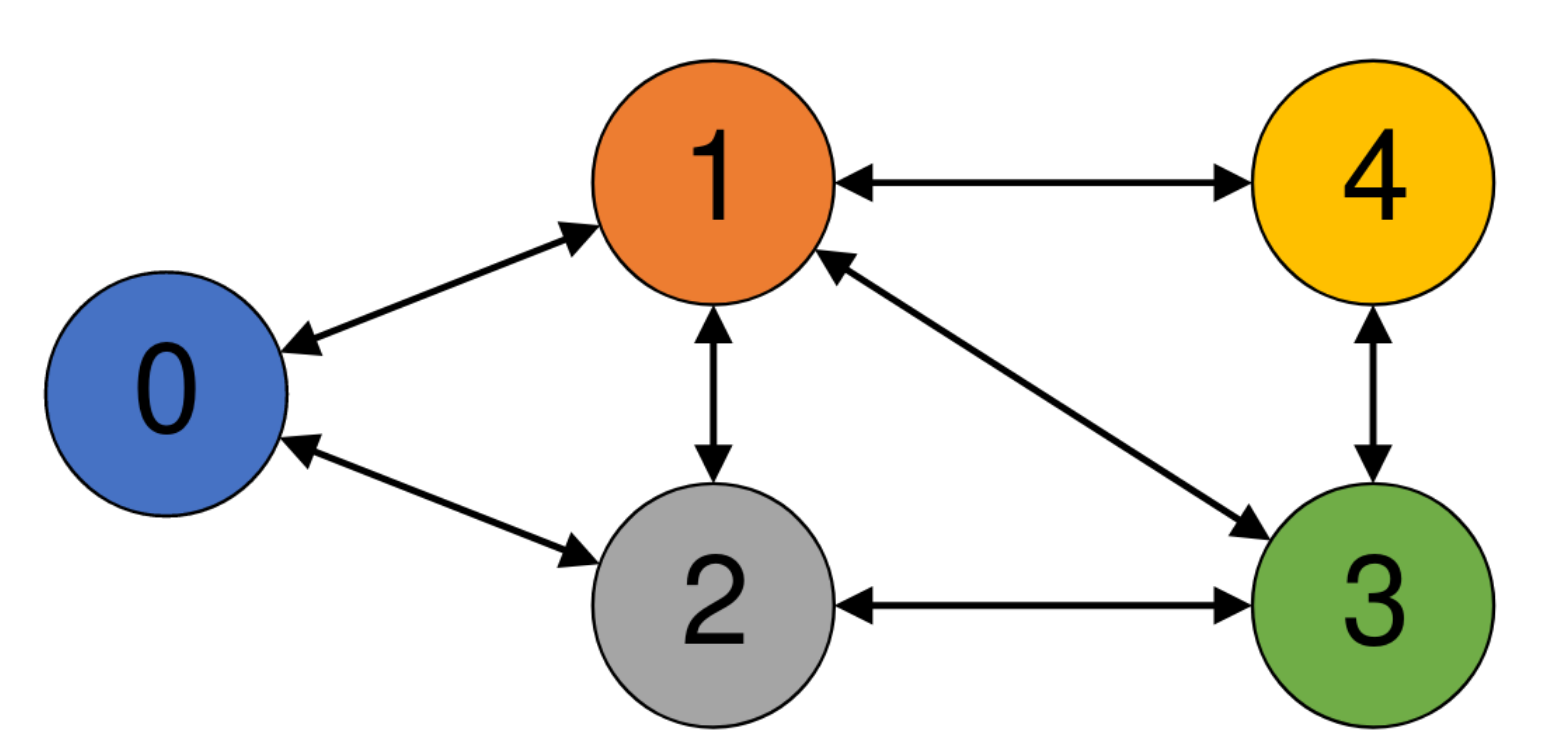
\includegraphics[width=\textwidth]{figures/graph.png}
                \caption{Graph}
            \end{subfigure}
            \hfill
            \begin{subfigure}[b]{0.47\textwidth}
                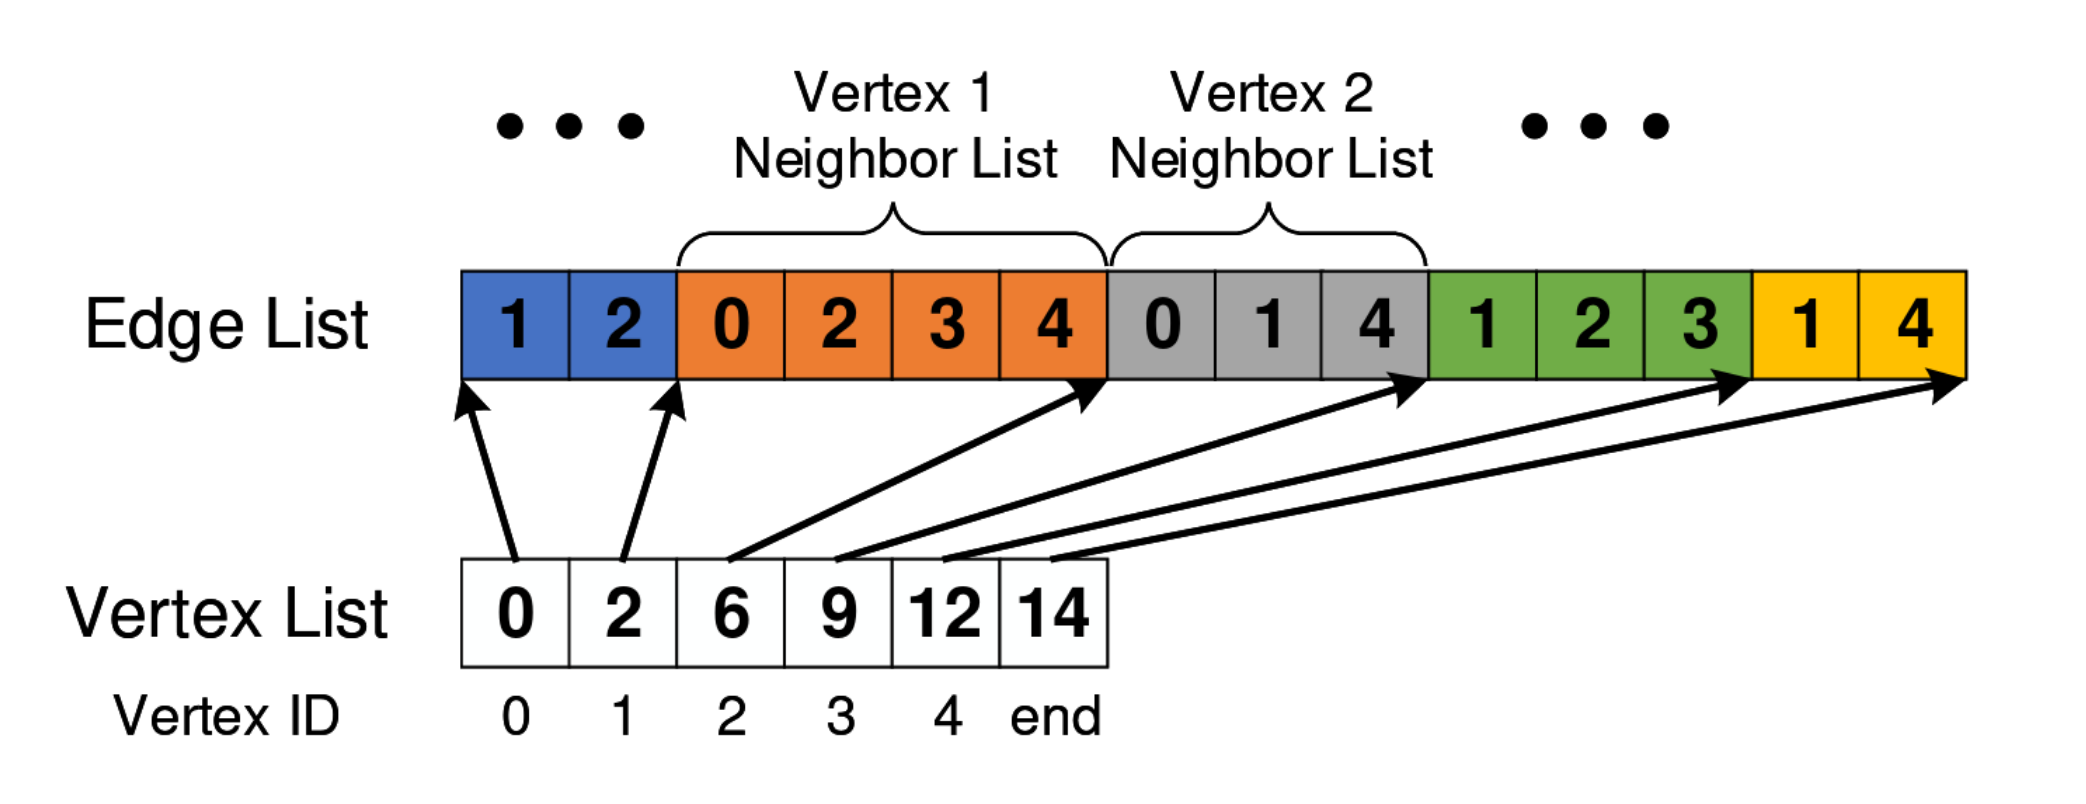
\includegraphics[width=\textwidth]{figures/csr_matrix.png}
                \caption{CSR matrix}
            \end{subfigure}
            \caption{Sample directed graph and its CSR adjacency matrix}
        \end{figure}
    \end{minipage}\hfill
\end{frame}

\begin{frame}[fragile] \frametitle{Проблема}
    \begin{itemize}
        \item Большинство реальных данных не помещается полностью в видеопамять GPU 
        \item Данные сильно разрежены, средняя степень вершины 71
        \item UVM влечет избыточное количество I/O операций
        {
            \begin{itemize}
                \item Слабая локальность реальных данных
                \item Размер страницы 4KB
                \item Копирование большого количества данных при сравнительно небольших запросах
            \end{itemize}
        }
        \item Необходима реструктуризация данных
        {
            \begin{itemize}
                \item Дополнительное время и ресурсы на выполнение
                \item Дополнительные усилия со стороны программиста 
            \end{itemize}
        }
    \end{itemize}
\end{frame}

\begin{frame}[fragile] \frametitle{Решение}
    \begin{itemize}
        \item Zero-copy, или \textit{direct access}
        \item Не требуется предварительная обработка данных
        \item Граф представляется в виде CSR матрицы смежности
        \item $|E| \ll |V|^2$
        \item Размер графа много больше доступной видеопамяти
    \end{itemize}
\end{frame}

\begin{frame}[fragile] \frametitle{Предварительные знания}
    \begin{itemize}
        \item Peripheral Component Interconnect Express (PCIe) --- стандарт высокоскоростной шины расширения для последовательной передачи данных
        \item Физическая топология --- звезда
        \item Программная топология --- шина
        \item Независимая передача данных в обе стороны 
        \item Распространенный интерфейс на материнских платах для подключения графических адаптеров, внешних накопителей, Wi-Fi и Ethernet компонент
    \end{itemize}
\end{frame}

\begin{frame}[fragile] \frametitle{Предварительные знания}
    \begin{center}
    \begin{minipage}[m]{0.75\linewidth}
        \begin{figure}
            \centering
            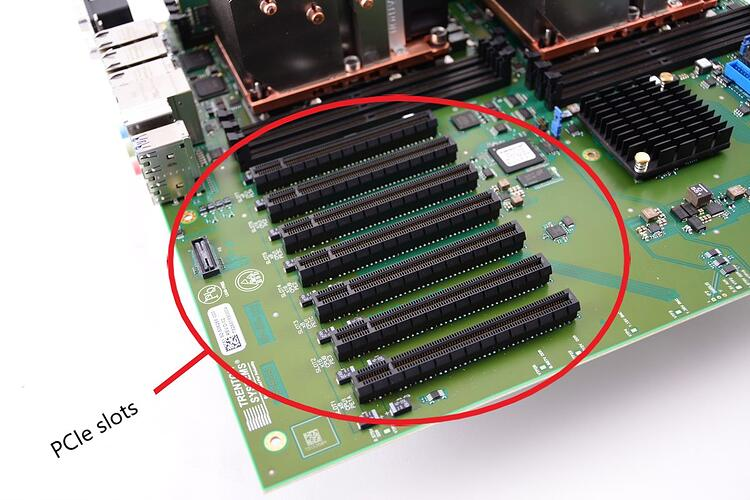
\includegraphics[width=\textwidth]{figures/pcie.jpg}
            \caption{PCIe slots located on the motherboard}
            \label{fig:pcie}
        \end{figure}
    \end{minipage}\hfill
    \end{center}
\end{frame}

\begin{frame}[fragile] \frametitle{Zero-copy: концепция}
    \begin{itemize}
        \item Доступ к zero-copy региону памяти осуществляется так, словно это глобальный регион памяти GPU
        \item GPU \textit{под капотом} преобразует запрос к этому региону и направляет его через внешний интерфейс, например PCIe, в систему
        \item На запрос может ответить любое устройство, которое способно отображать свои регионы памяти (\textit{memory-map}) в пространство адресов транспортной шины, т.е. PCIe интерфейса, например
    \end{itemize}
\end{frame}

\begin{frame}[fragile] \frametitle{Zero-copy: пример}
    \begin{center}
    \begin{minipage}[m]{0.95\linewidth}
        \begin{figure}
            \centering
            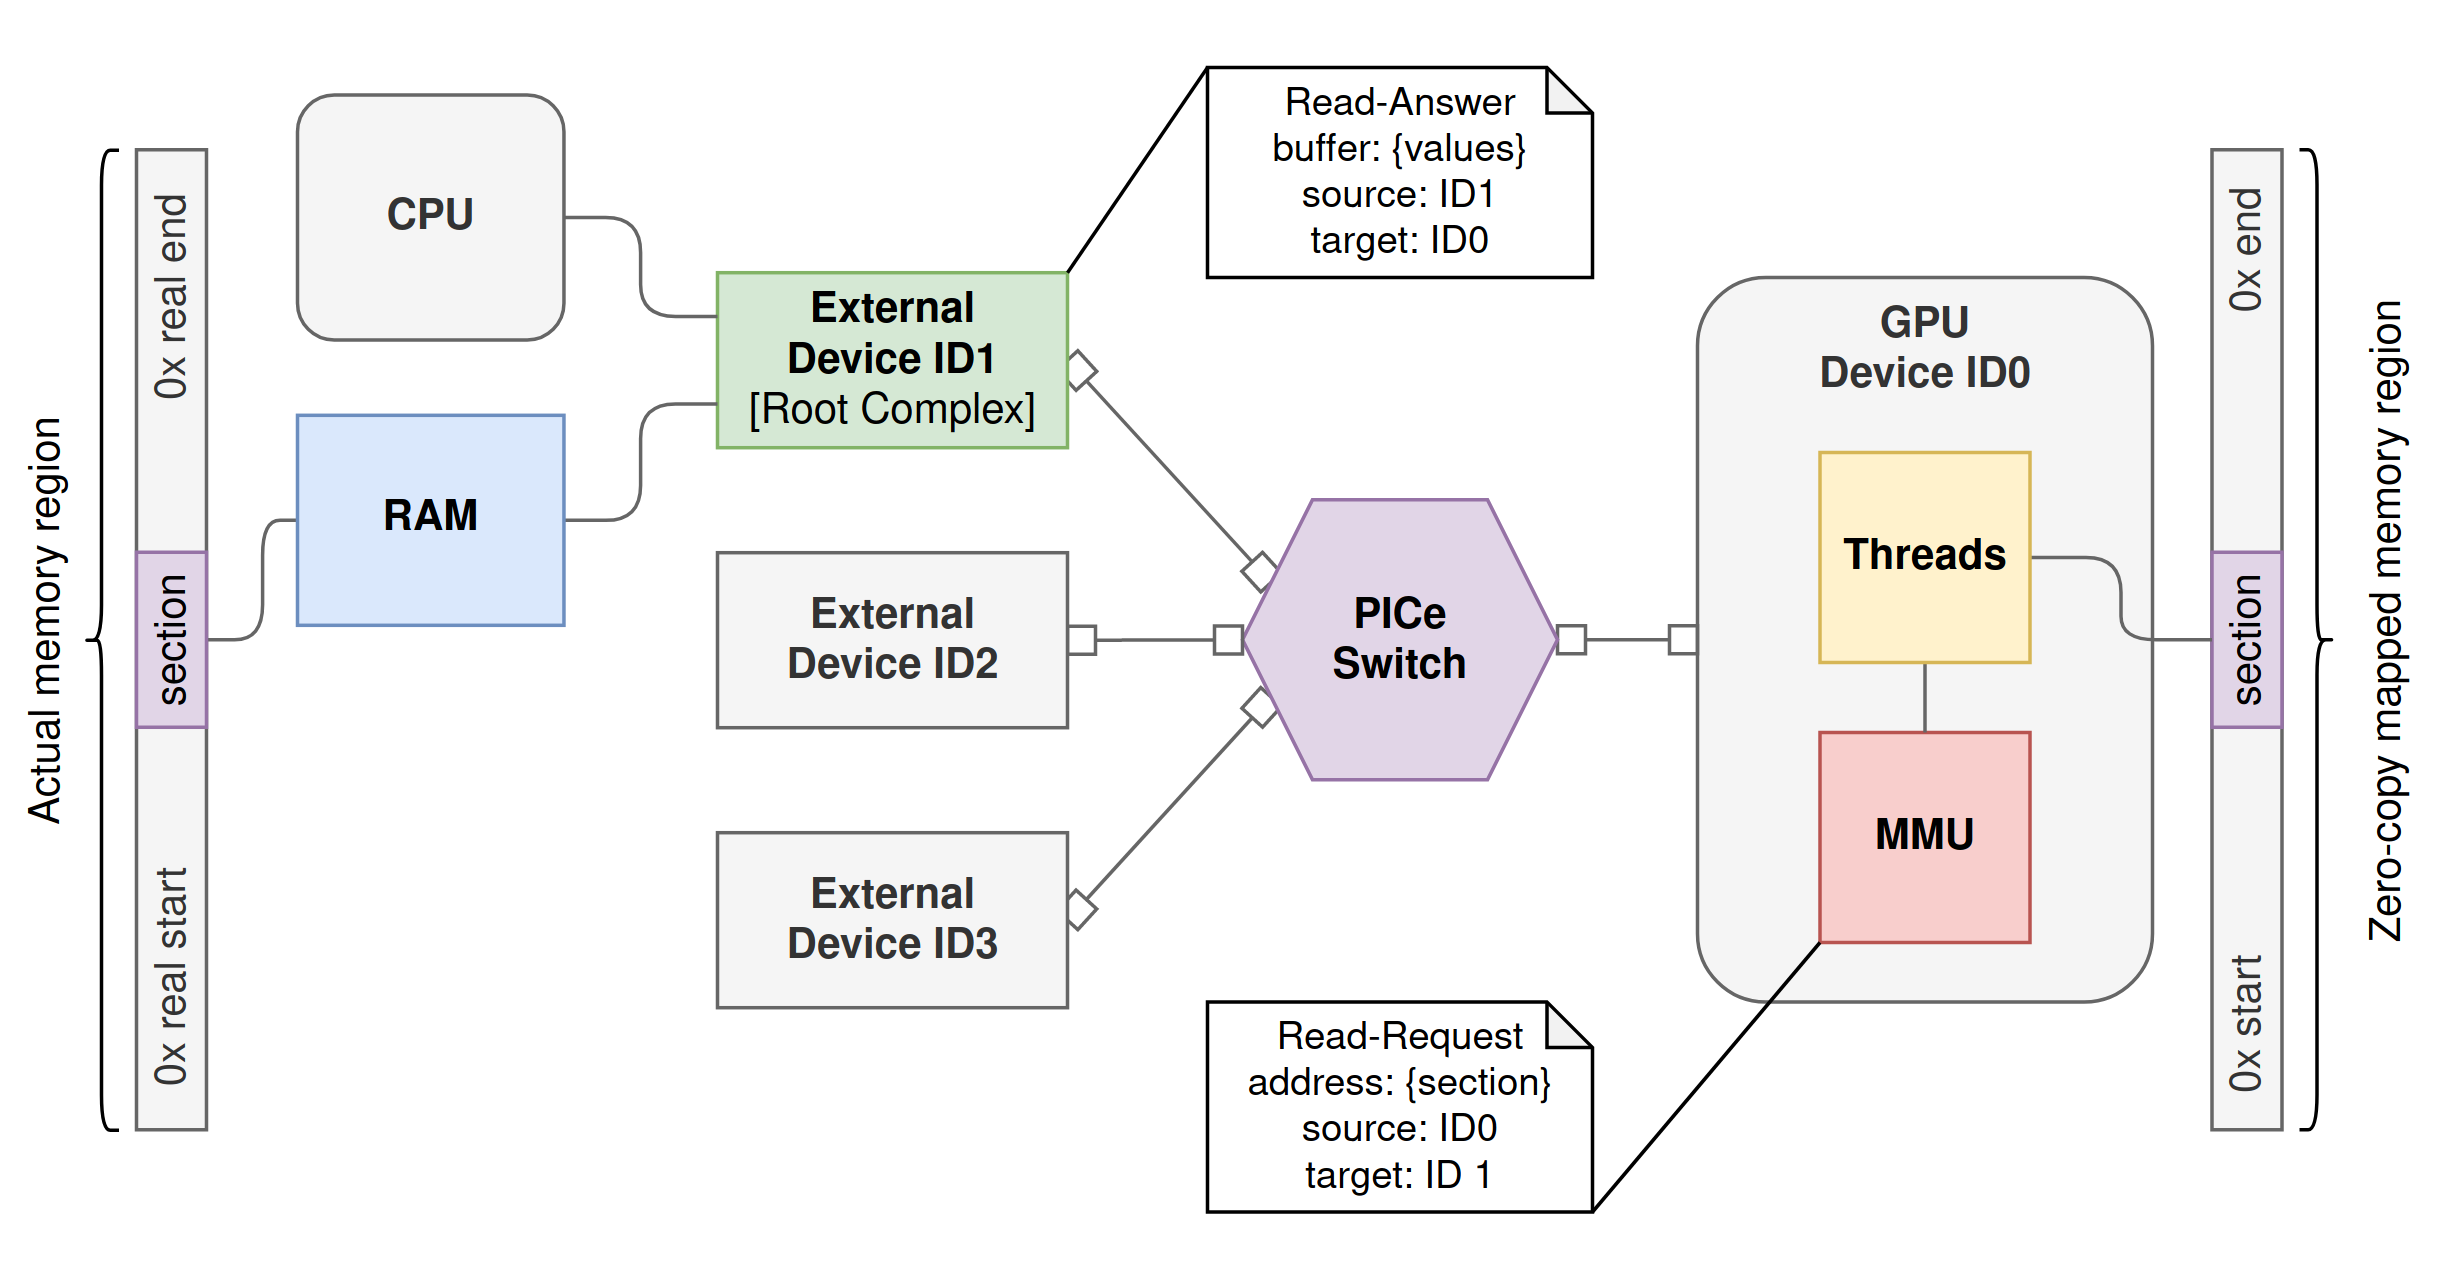
\includegraphics[width=\textwidth]{figures/zero_copy.png}
            \caption{Zero-copy mechanism with PCIe}
            \label{fig:zero_copy}
        \end{figure}
    \end{minipage}\hfill
    \end{center}
\end{frame}

\begin{frame}[fragile] \frametitle{Zero-copy: механизм}
     \begin{itemize}
         \item С точки зрения системы
         {
            \begin{itemize}
                \item Выделить требуемый буфер в оперативной (\textit{host}) памяти
                \item Закрепить (\textit{pinning}) буфер в памяти, т.е.запретить перемещение или вытеснение страниц этого региона 
                \item Отобразить адреса буфера в таблицу страниц GPU
                \item Получить адрес буфера для использования в GPU ядрах
            \end{itemize}
         }
         \item С точки зрения \textbf{CUDA API}
         {
            \begin{itemize}
                \item Выделить память с помощью \\ \textit{cudaError\_t cudaMallocHost(void** ptr, size\_t size)}
                \item Описание функции: allocates size bytes of host memory that is page-locked and accessible to the device. Since the memory can be accessed directly by the device, it can be read or written with much higher bandwidth than pageable memory obtained with functions such as malloc().
            \end{itemize}
         }
     \end{itemize}
\end{frame}

\begin{frame}[fragile] \frametitle{Монитор трафика}
    \begin{center}
    \begin{minipage}[m]{0.95\linewidth}
        \begin{figure}
            \centering
            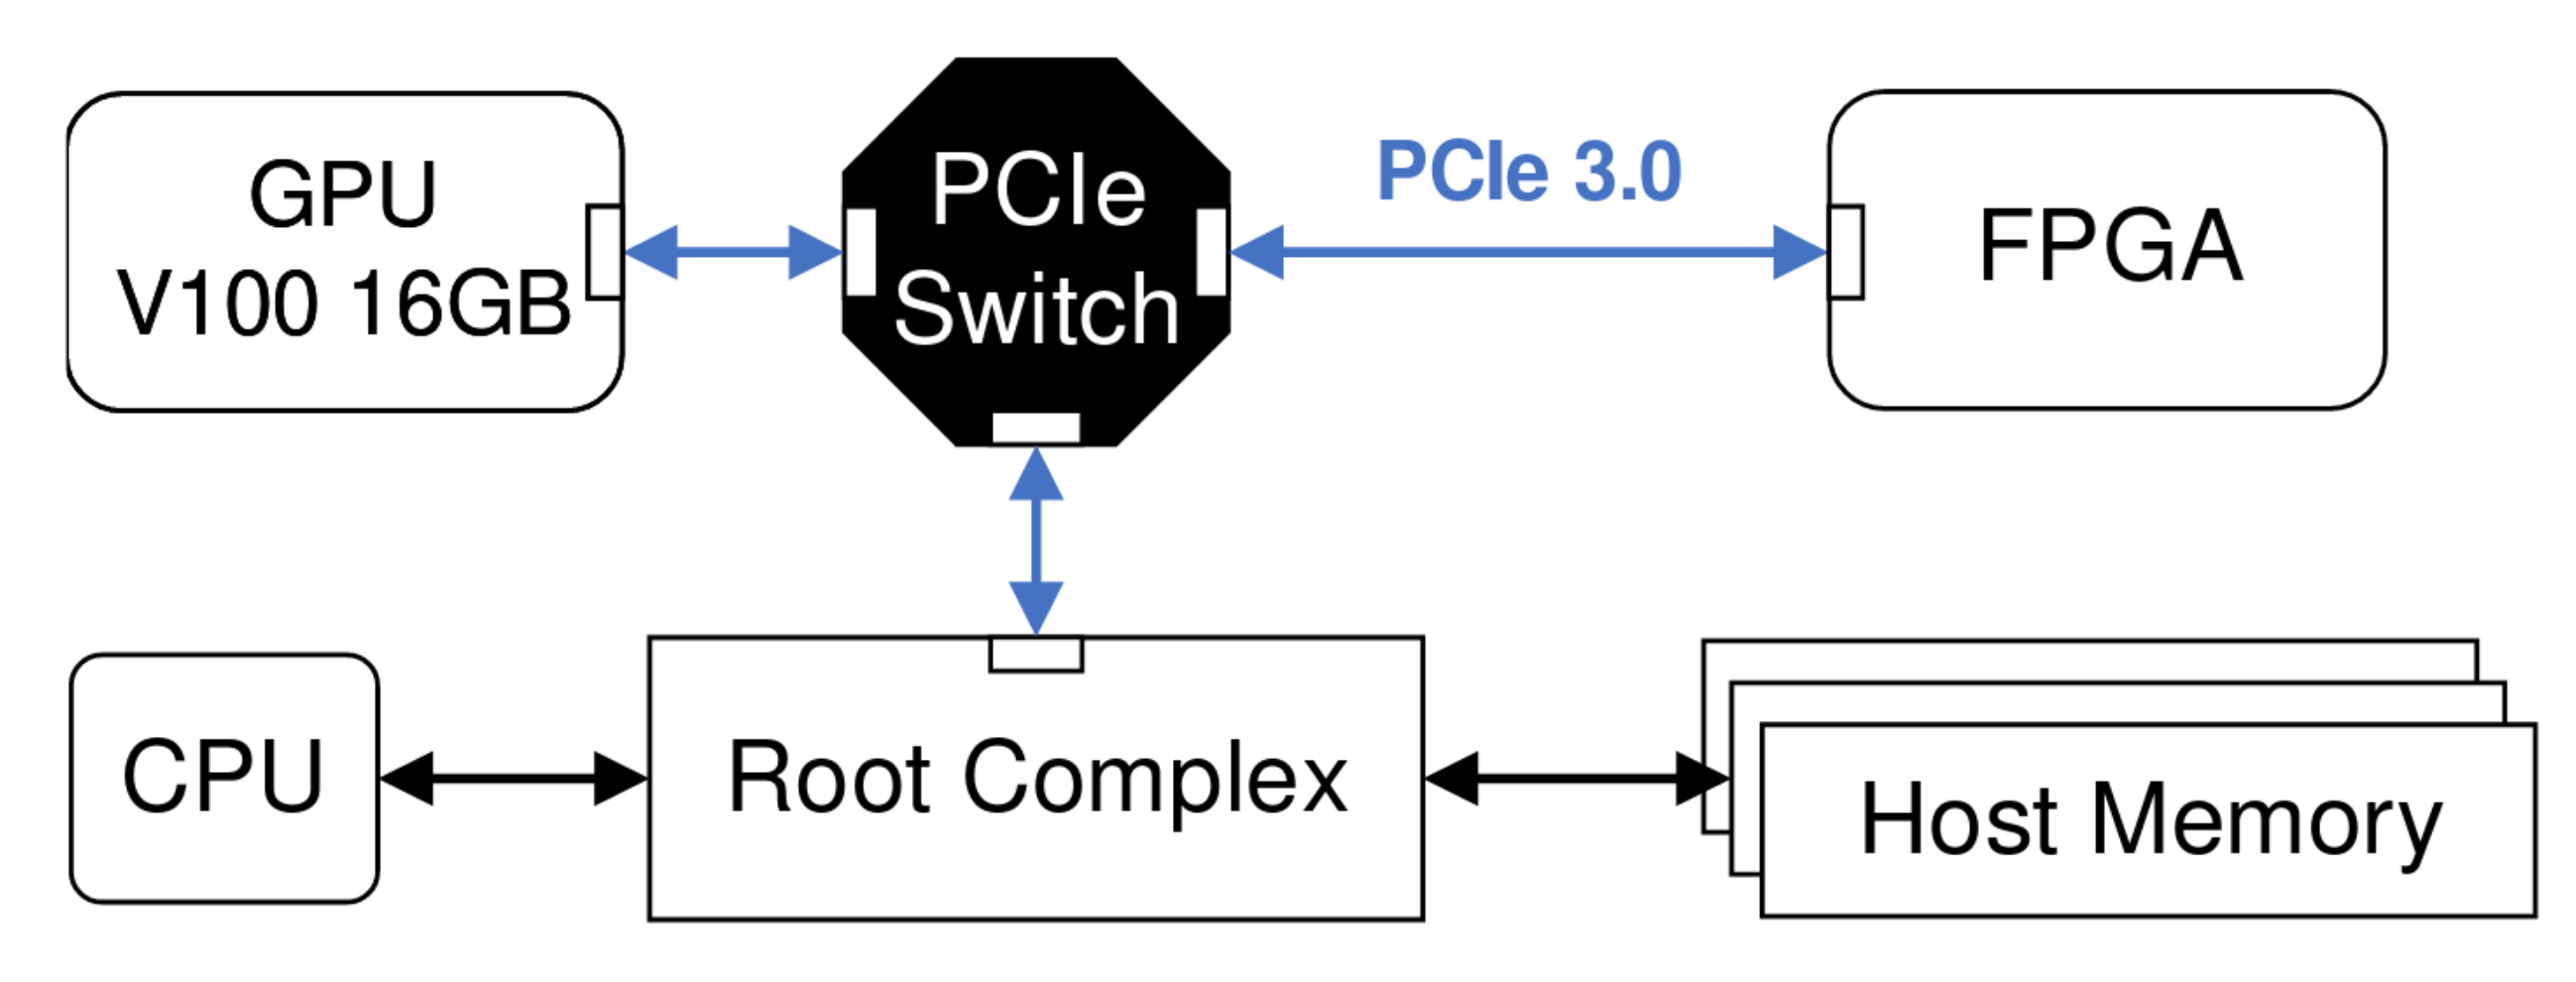
\includegraphics[width=\textwidth]{figures/monitor_schema.png}
            \caption{PCIe traffic monitoring environment. The FPGA is used to characterize the zero-copy memory access pattern from GPU}
            \label{fig:monitor_schema}
        \end{figure}
    \end{minipage}\hfill
    \end{center}
\end{frame}

\begin{frame}[fragile] \frametitle{Паттерны доступа}
    \begin{minipage}[m]{1.0\linewidth}
        \begin{figure}
            \centering
            \begin{subfigure}[b]{0.3\textwidth}
                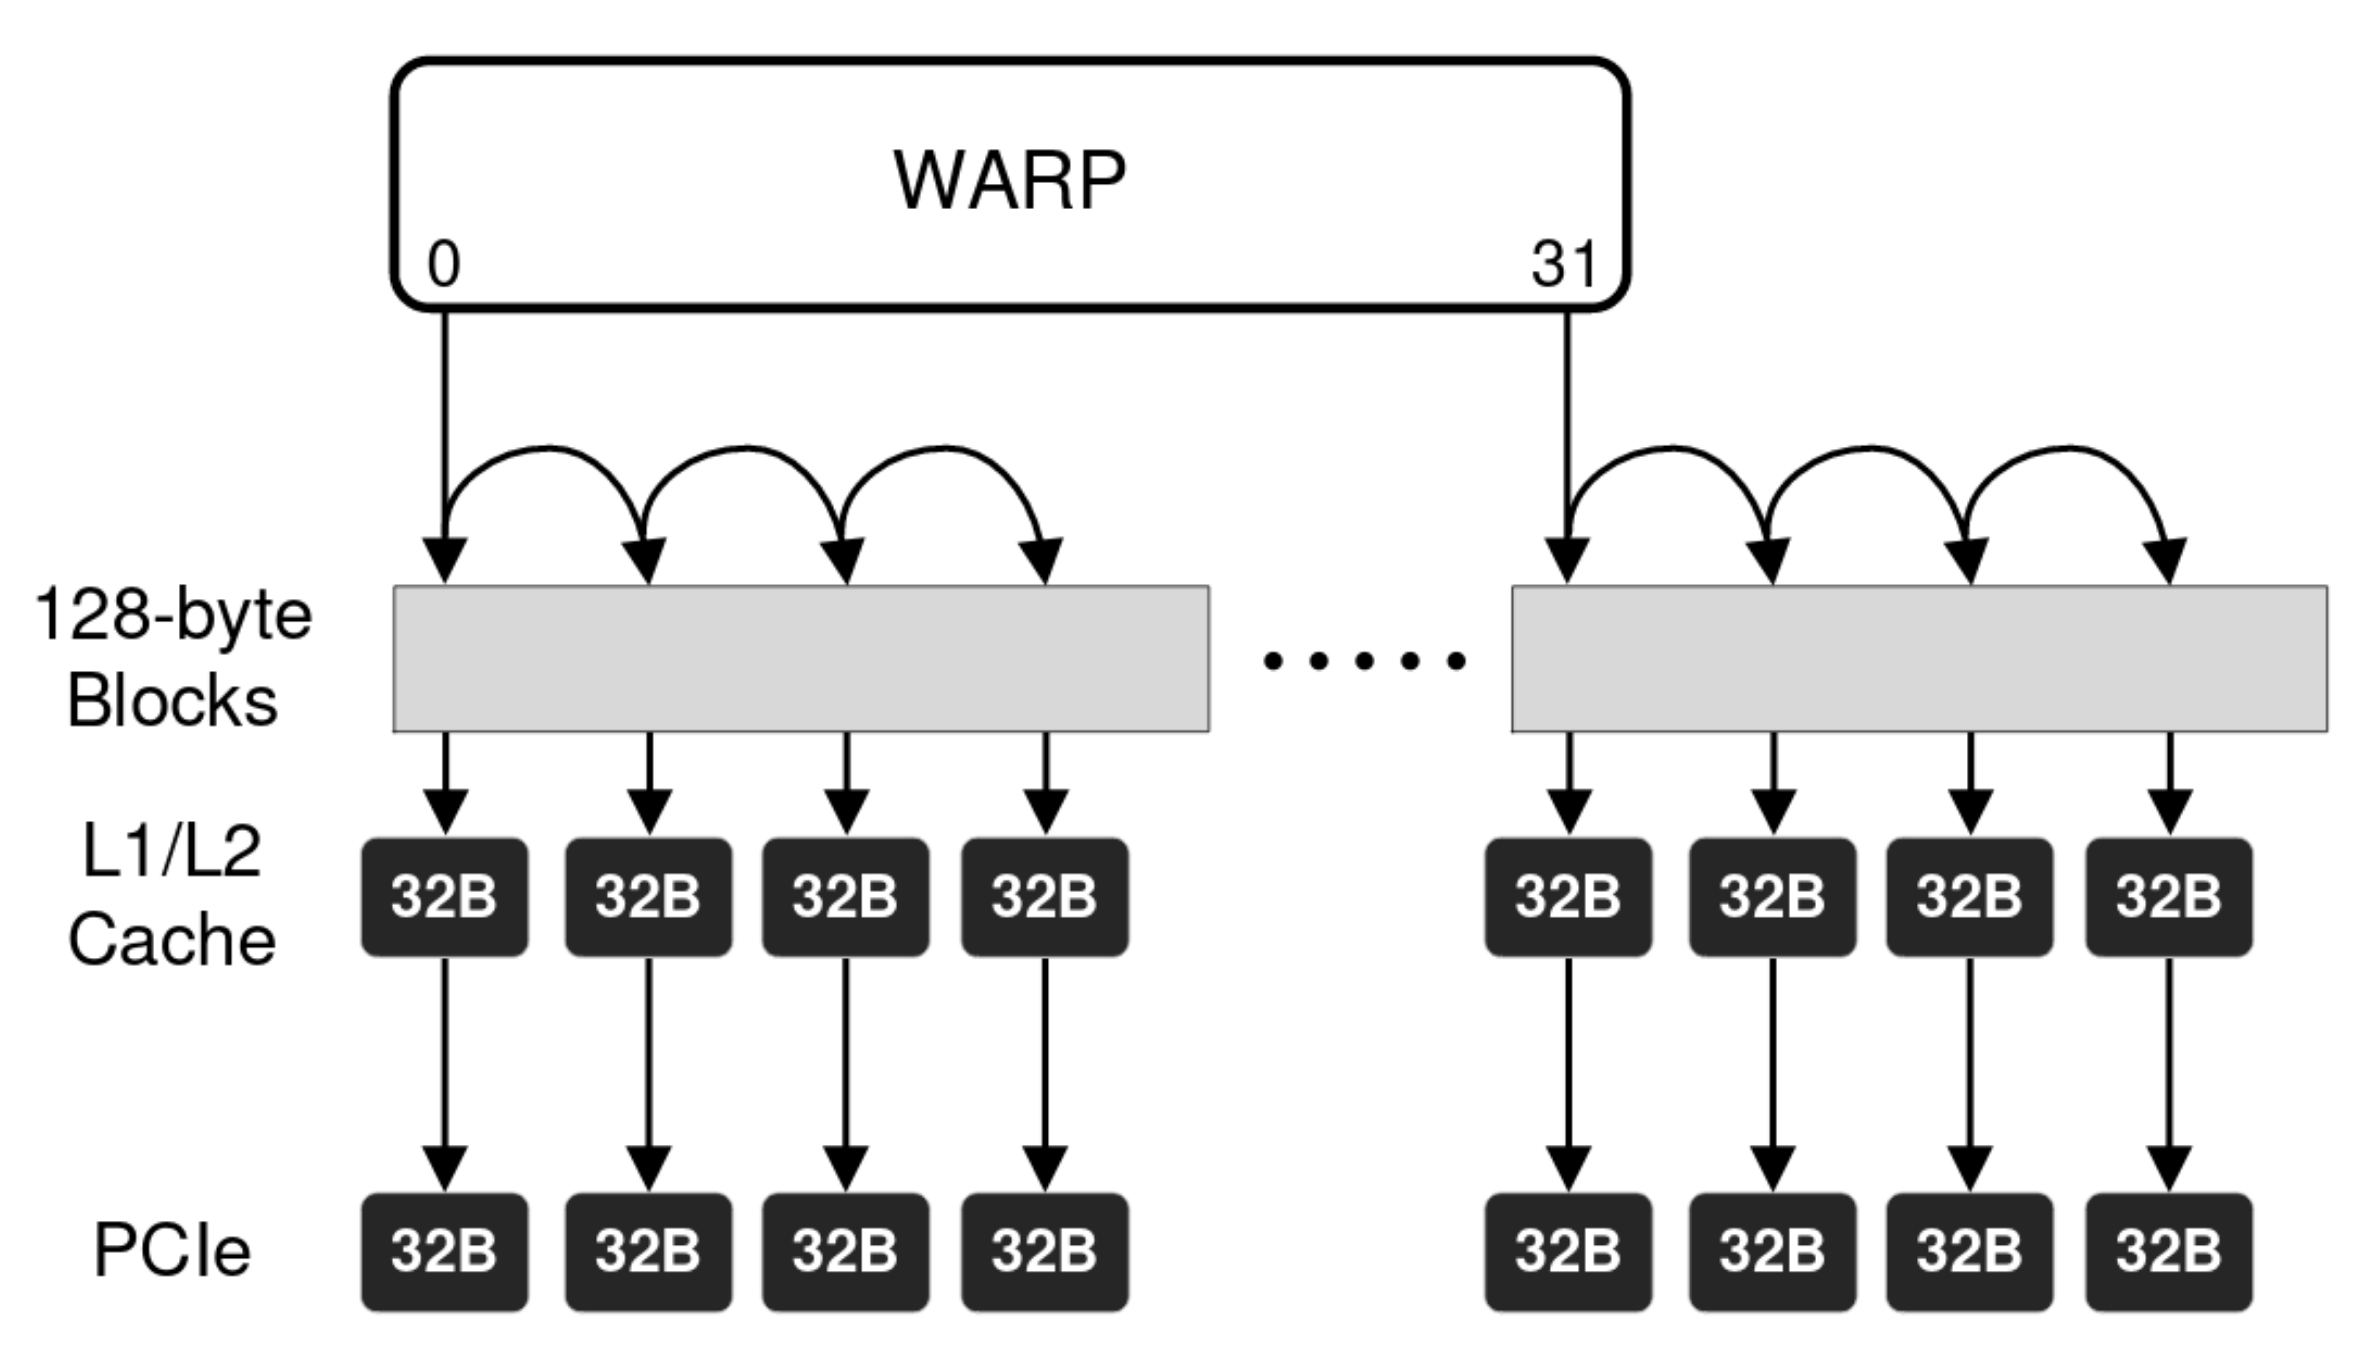
\includegraphics[width=\textwidth]{figures/strided_access.png}
                \caption{Strided}
            \end{subfigure}
            \hfill
            \begin{subfigure}[b]{0.3\textwidth}
                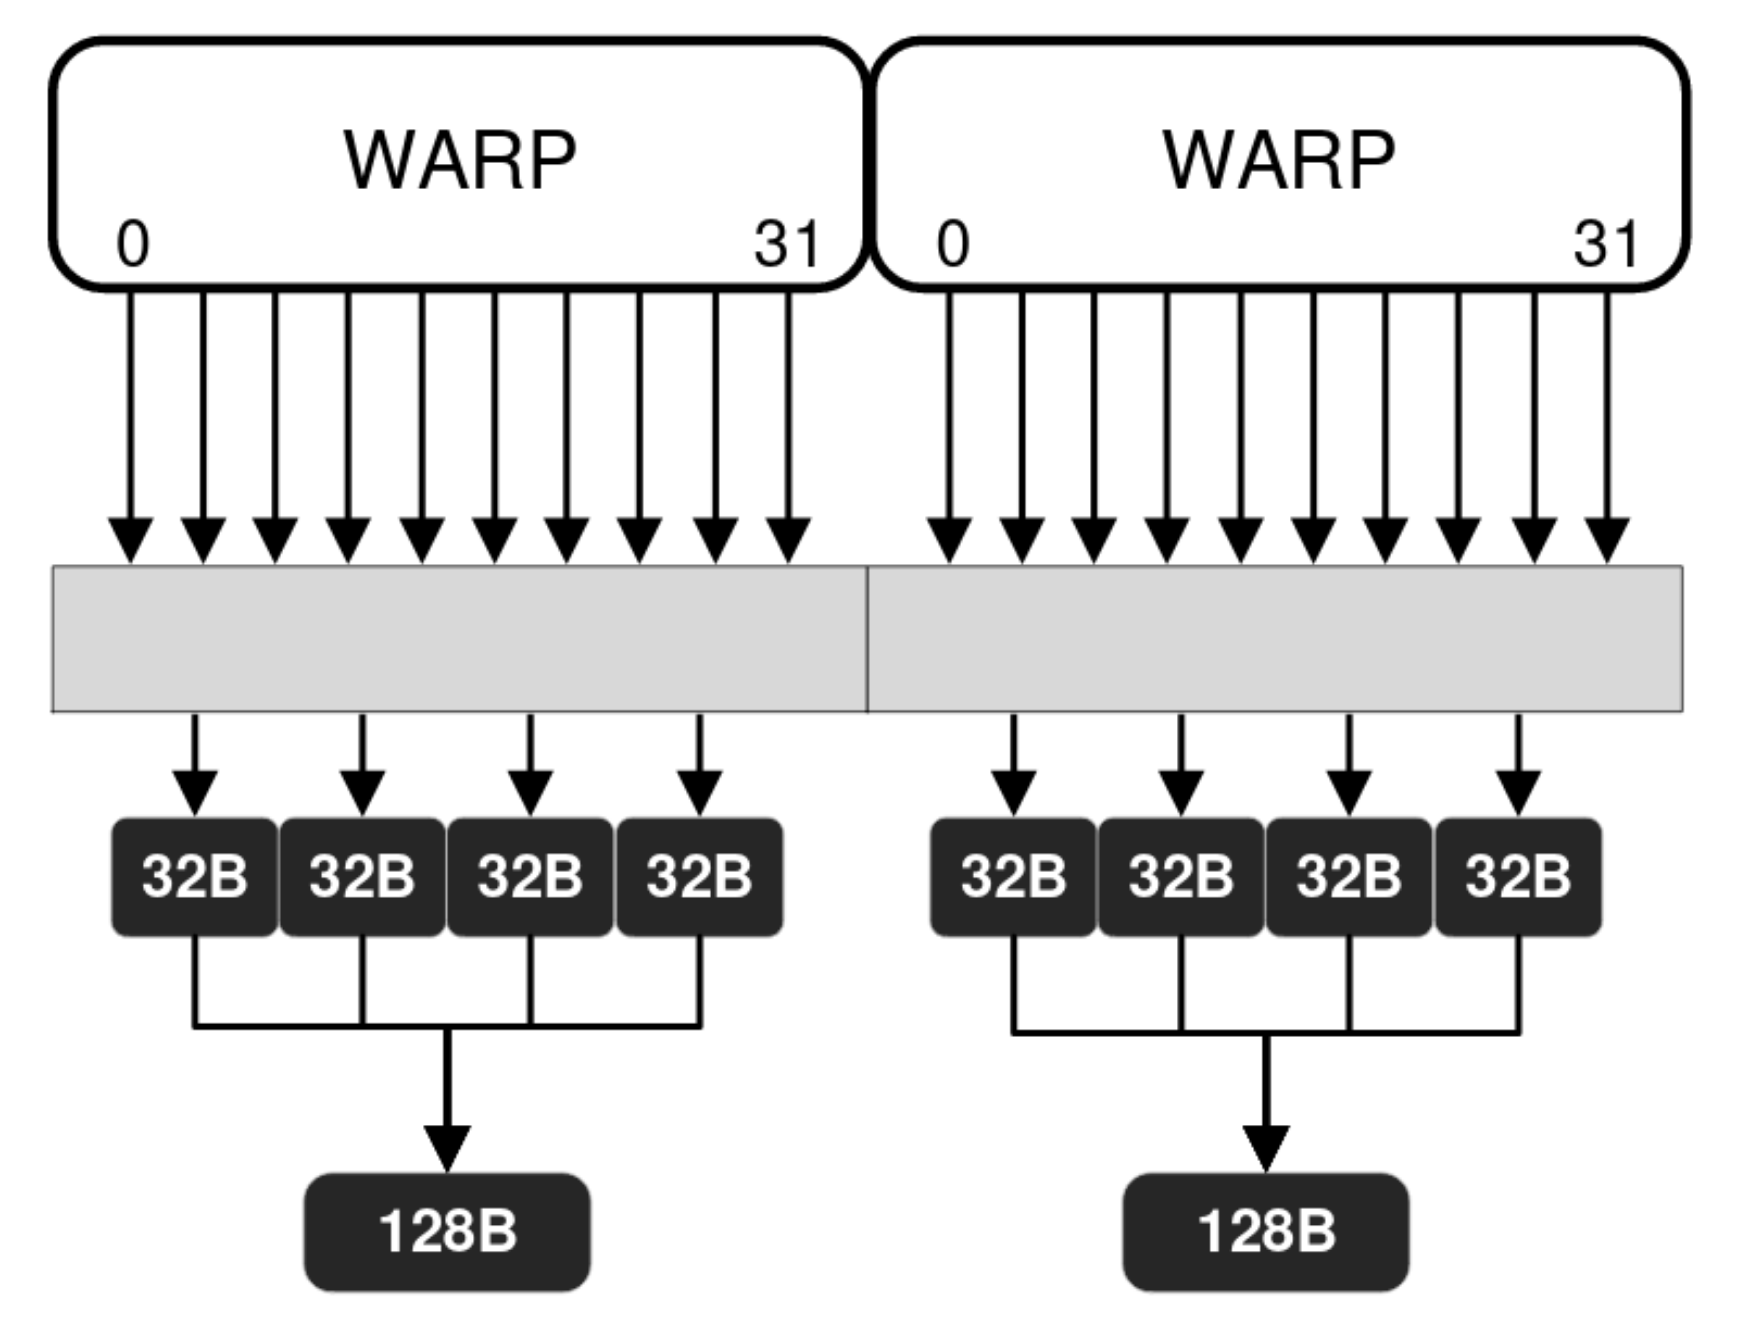
\includegraphics[width=\textwidth]{figures/merged_aligned_access.png}
                \caption{Merged and Aligned}
            \end{subfigure}
            \hfill
            \begin{subfigure}[b]{0.3\textwidth}
                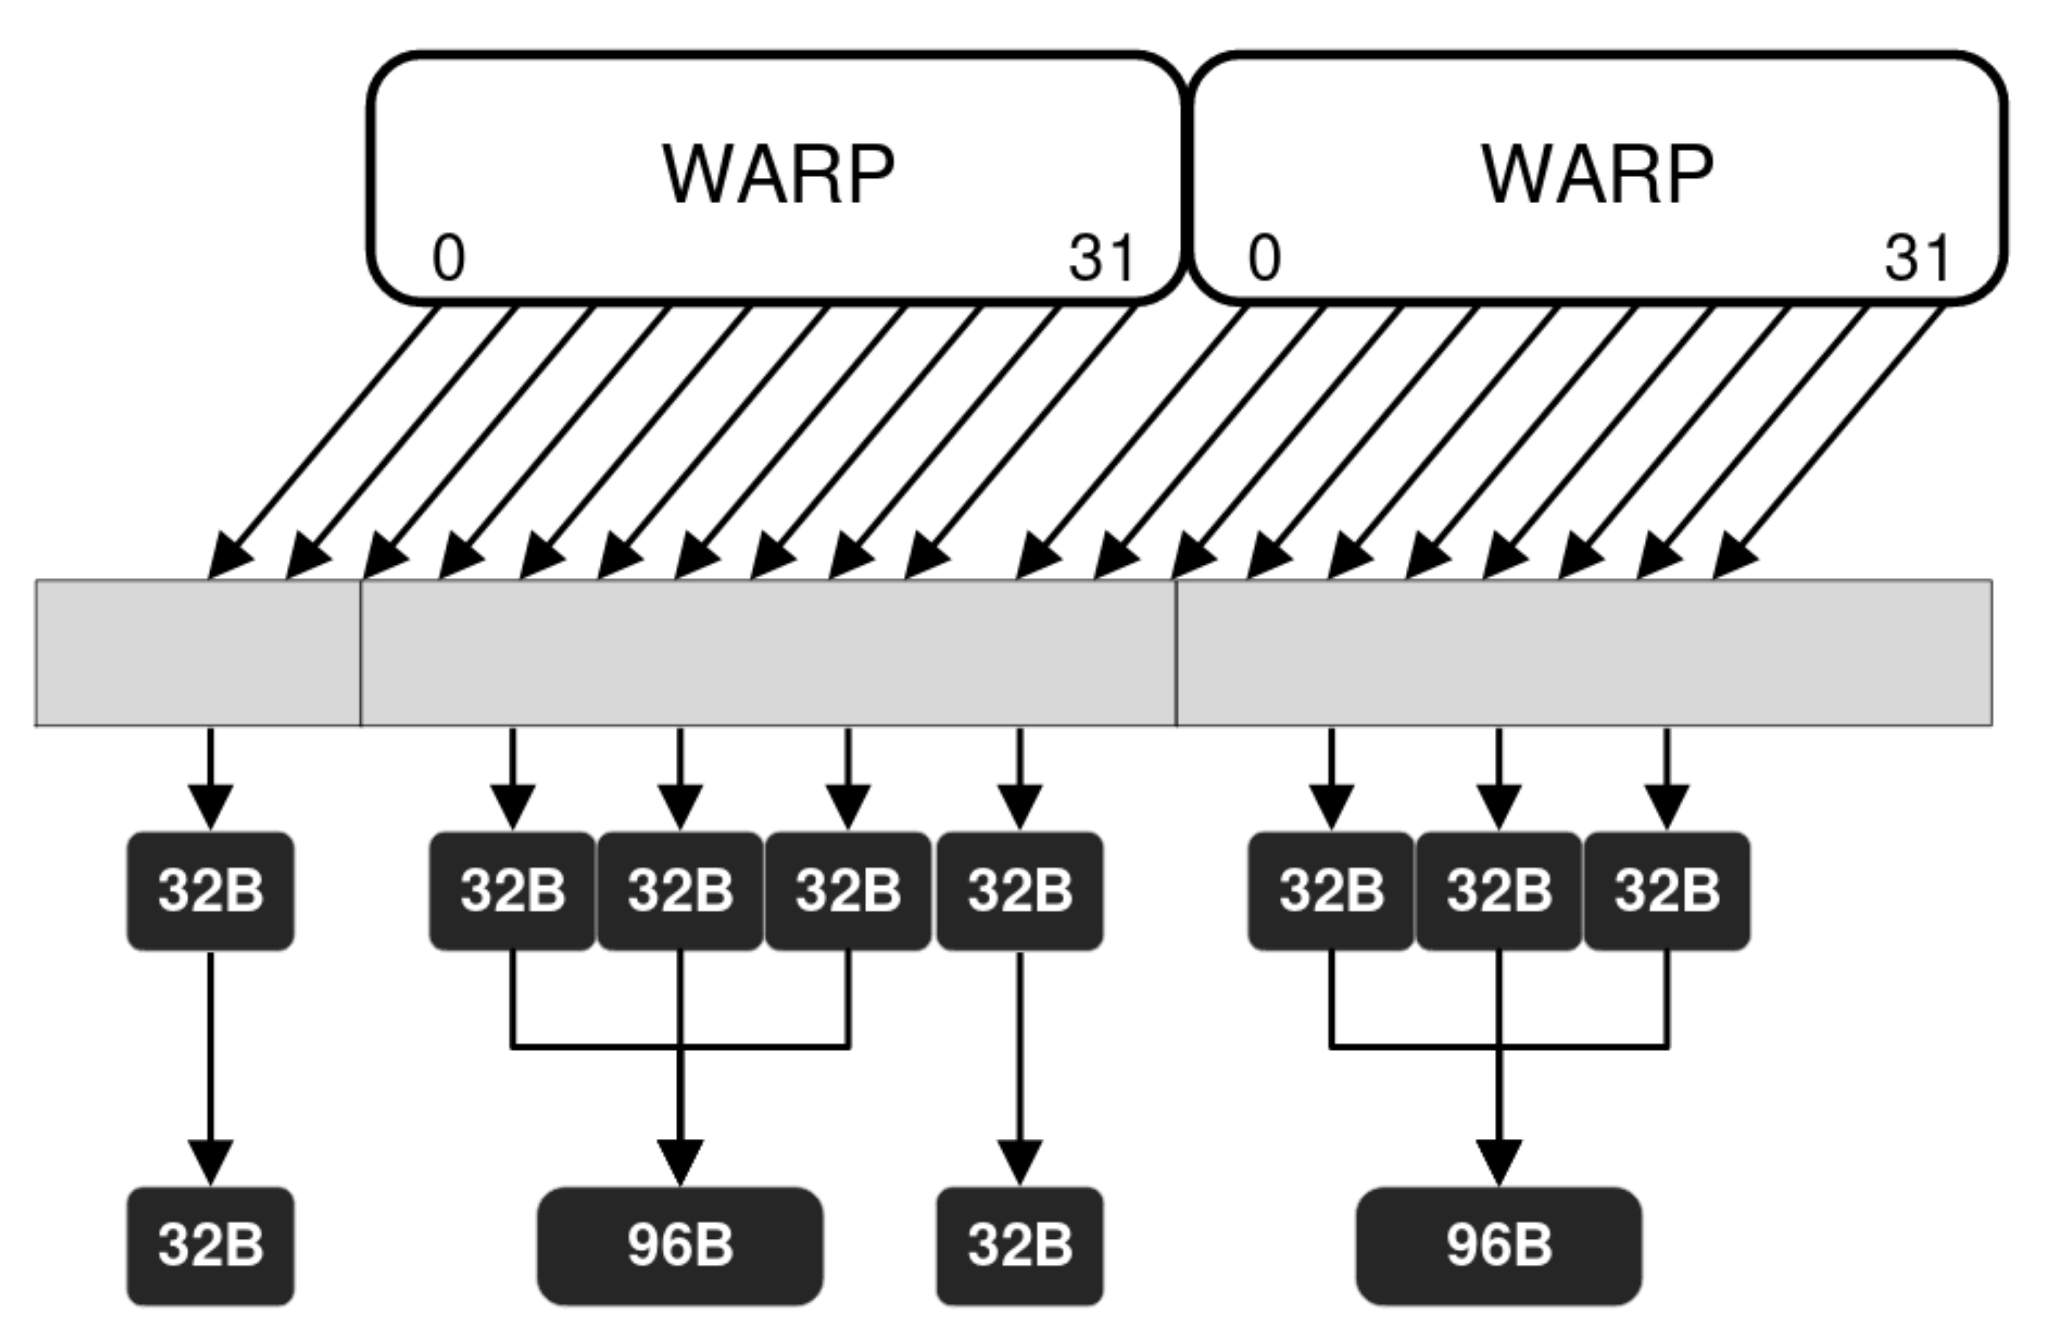
\includegraphics[width=\textwidth]{figures/merged_misaligned_access.png}
                \caption{Merged but Misaligned}
            \end{subfigure}
            \caption{GPU PCIe memory request patterns observed with FPGA}
        \end{figure}
    \end{minipage}\hfill
\end{frame}

\begin{frame}[fragile] \frametitle{Исследование}
    \begin{itemize}
        \item Strided
        {
            \begin{itemize}
                \item Запросы размером 32 байта
                \item Размер заголовка PCIe 3.0 TLP пакета 18 байт, overhead 36\%
                \item Максимальная пропускная способность с RTT $1us$: 
                32 байта $/ 1us * 256 = 7.63 GB/s$ 
                \item Пропускная способность с RTT $1.6us$: $4.77GB/s$
                \item Минимальный запрос к DDR4 DRAM 64 байта
                \item Максимальная скорость DDR4 2400MHz DRAM $19.2GB/s$
                \item С учетом размера запроса в 32 байта: $9.6GB/s$
            \end{itemize}
        }
        \item Merged and Aligned
        {
            \begin{itemize}
                \item Запросы размером 128 байт
                \item Overhead заголовка PCIe TLP пакета: 12.3\%
                \item Достаточно, чтобы заполнить PCIe 3.0 канал в $16GB/s$ 
            \end{itemize}
        }
        \item Merged but Misaligned
        {
        }
    \end{itemize}
\end{frame}

\begin{frame}[fragile] \frametitle{Результаты}
    \begin{center}
    \begin{minipage}[m]{0.85\linewidth}
        \begin{figure}
            \centering
            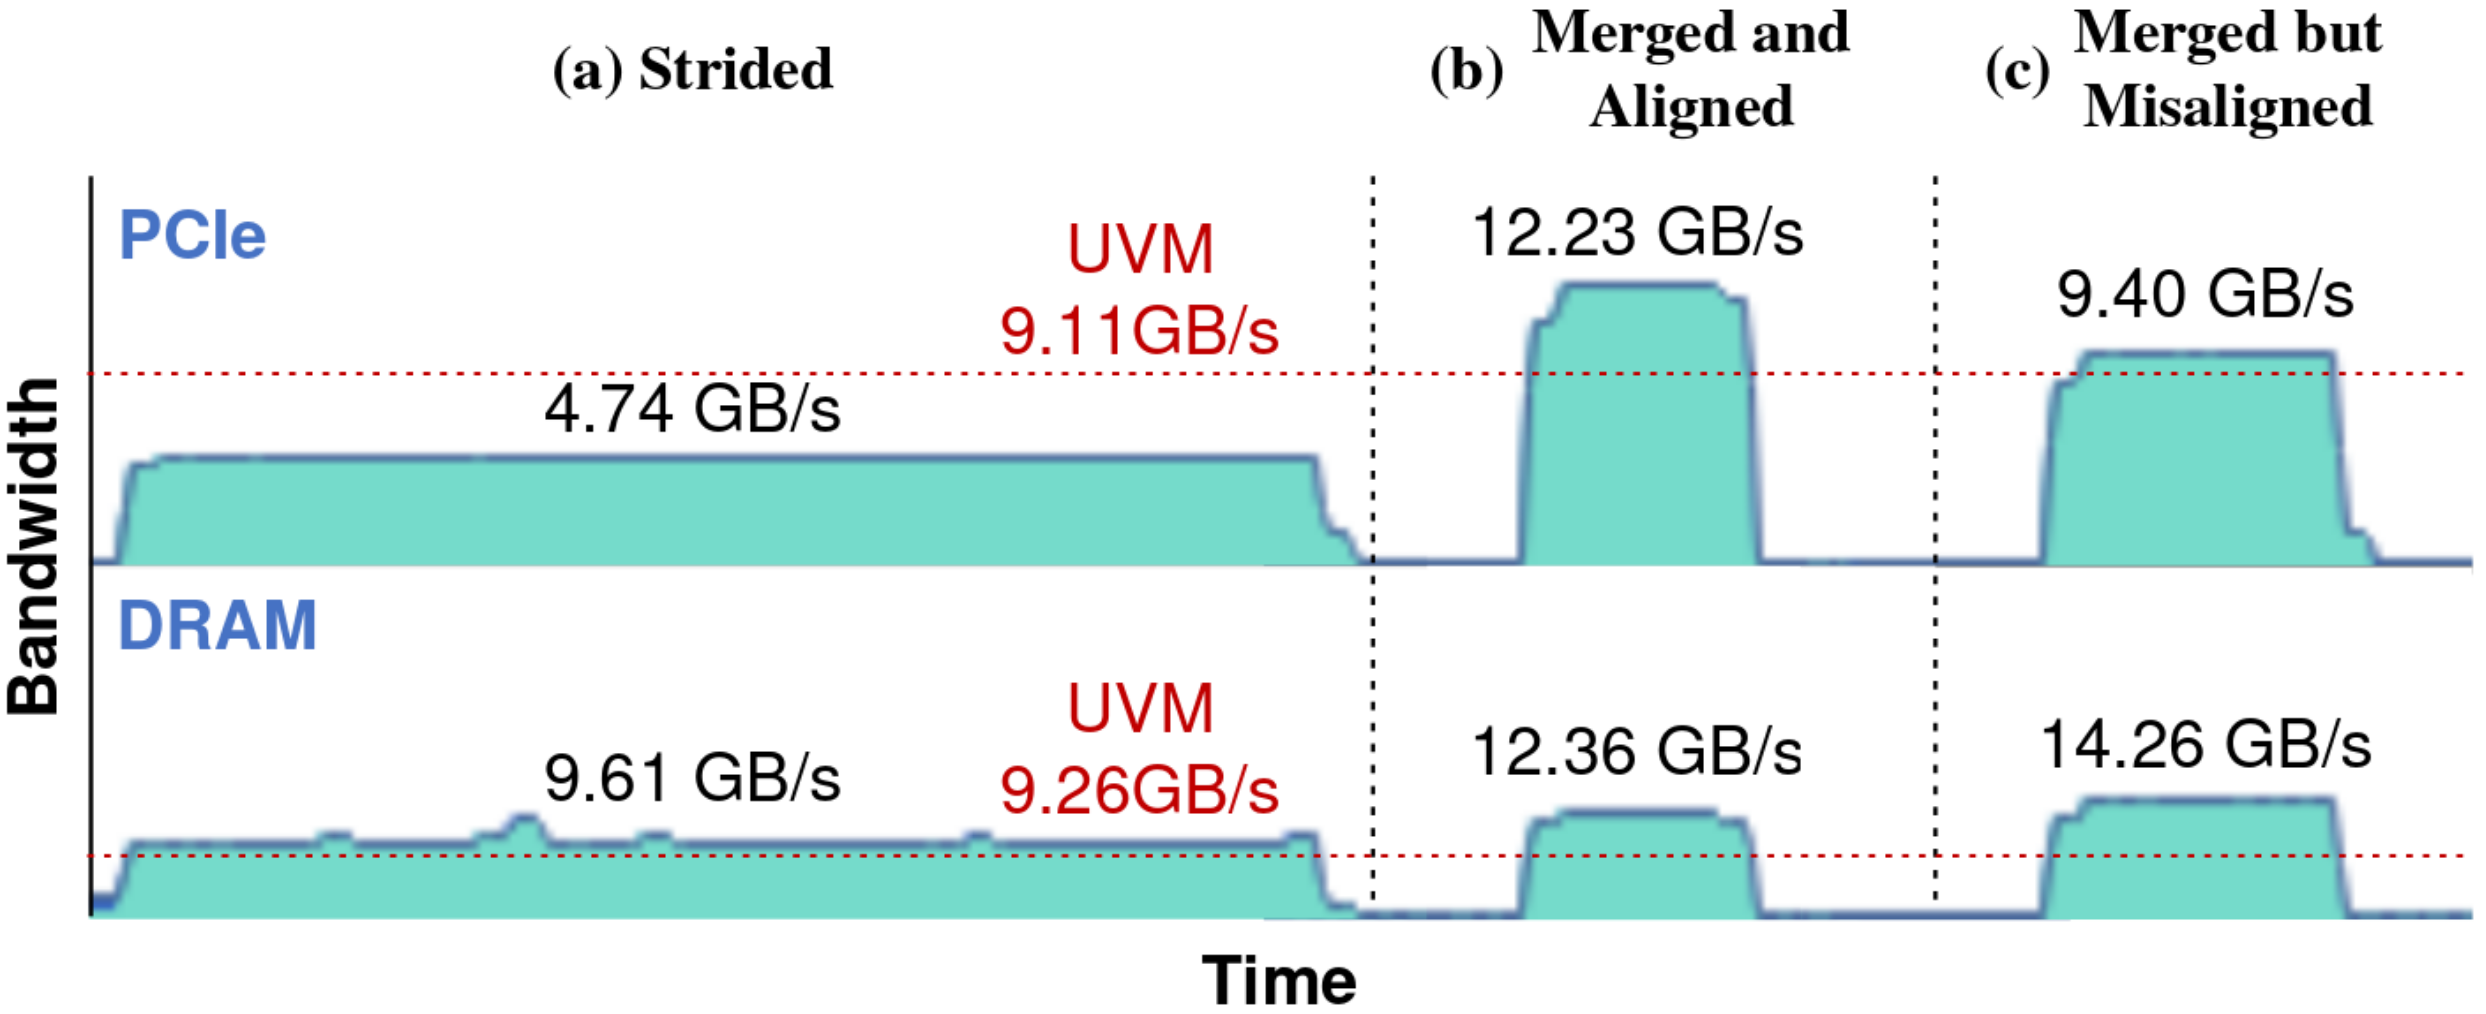
\includegraphics[width=\textwidth]{figures/access_patterns_utilization.png}
            \caption{Average PCIe and DRAM bandwidth utilization for the dif-ferent zero-copy access patterns}
            \label{fig:access_patterns_utilization}
        \end{figure}
    \end{minipage}\hfill
    \end{center} 
\end{frame}

\begin{frame}[fragile] \frametitle{EMOGI}
    \begin{minipage}[m]{1.0\linewidth}
        \begin{figure}
            \centering
            \begin{subfigure}[b]{0.44\textwidth}
                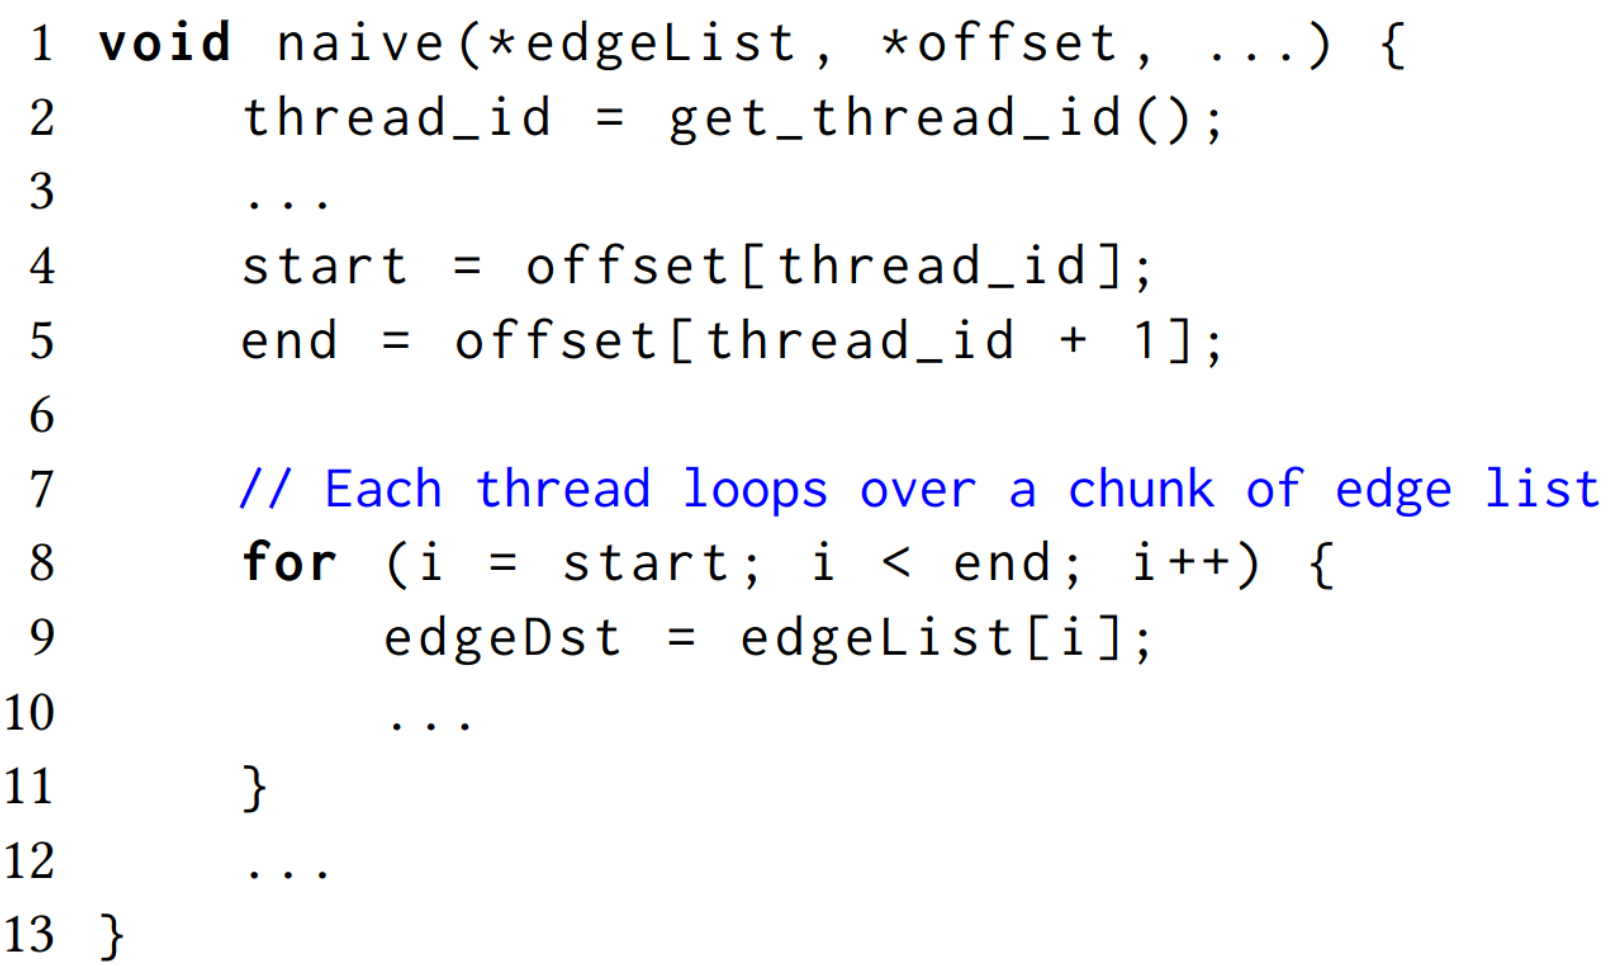
\includegraphics[width=\textwidth]{figures/emogi_naive.png}
                \caption{Na\"{\i}ve Uncoalesced Memory Access}
            \end{subfigure}
            \hfill
            \begin{subfigure}[b]{0.44\textwidth}
                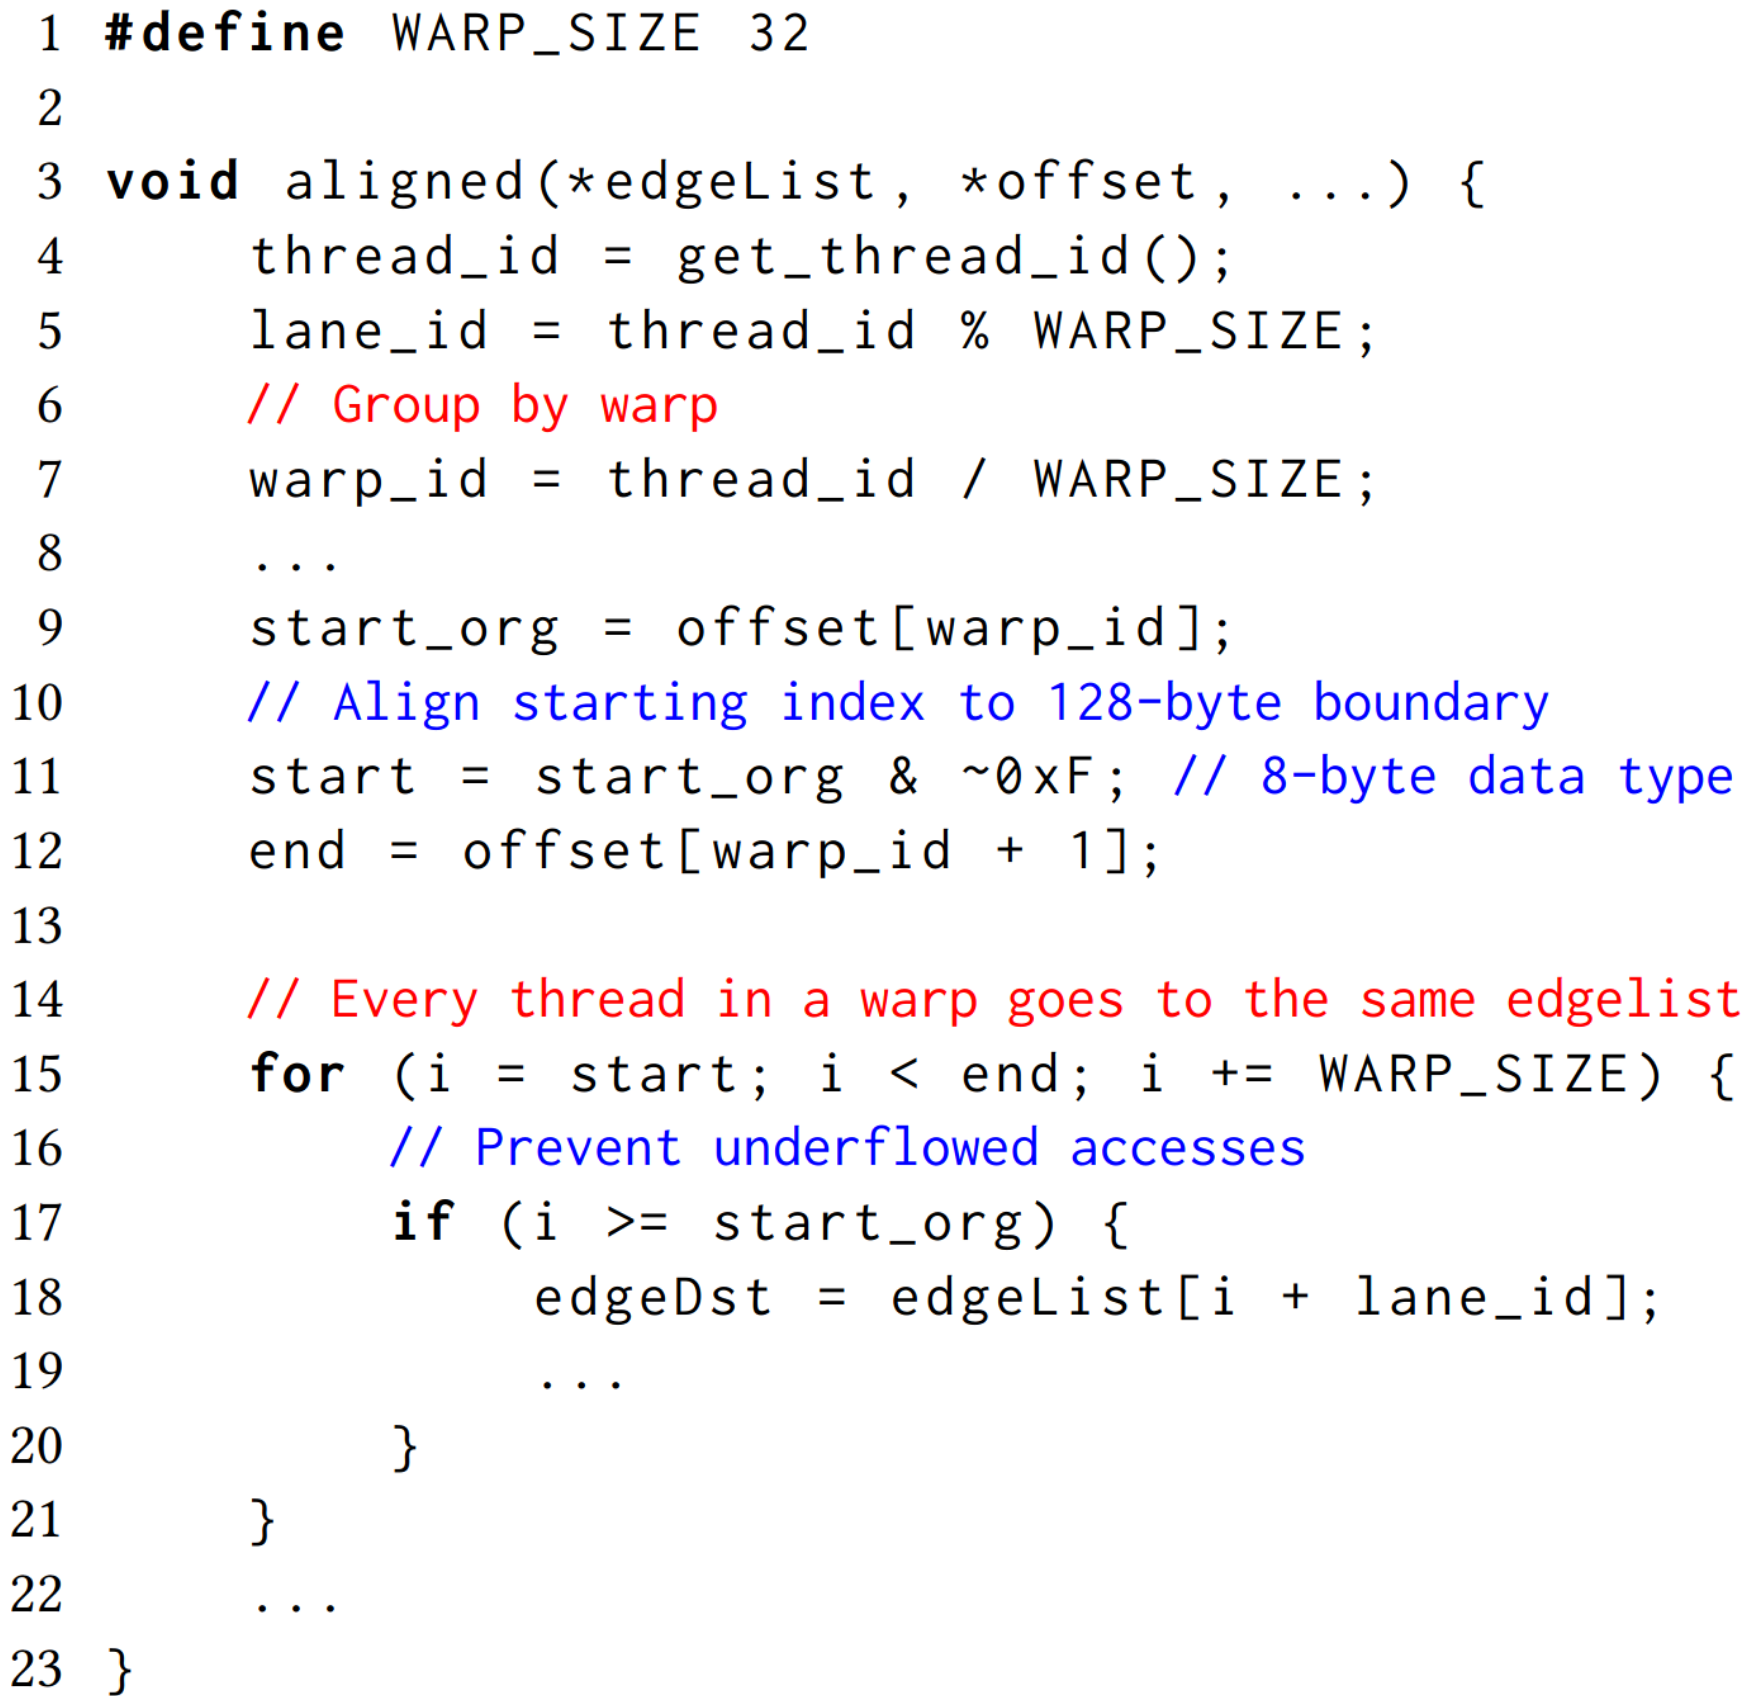
\includegraphics[width=\textwidth]{figures/emogi.png}
                \caption{EMOGI Coalesced Memory Access (Merged and Aligned)}
            \end{subfigure}
            \caption{Code listing for solution}
        \end{figure}
    \end{minipage}\hfill
\end{frame}

\begin{frame}[fragile] \frametitle{Эксперименты: система}
    \begin{center}
    \begin{minipage}[m]{0.95\linewidth}
        \begin{figure}
            \centering
            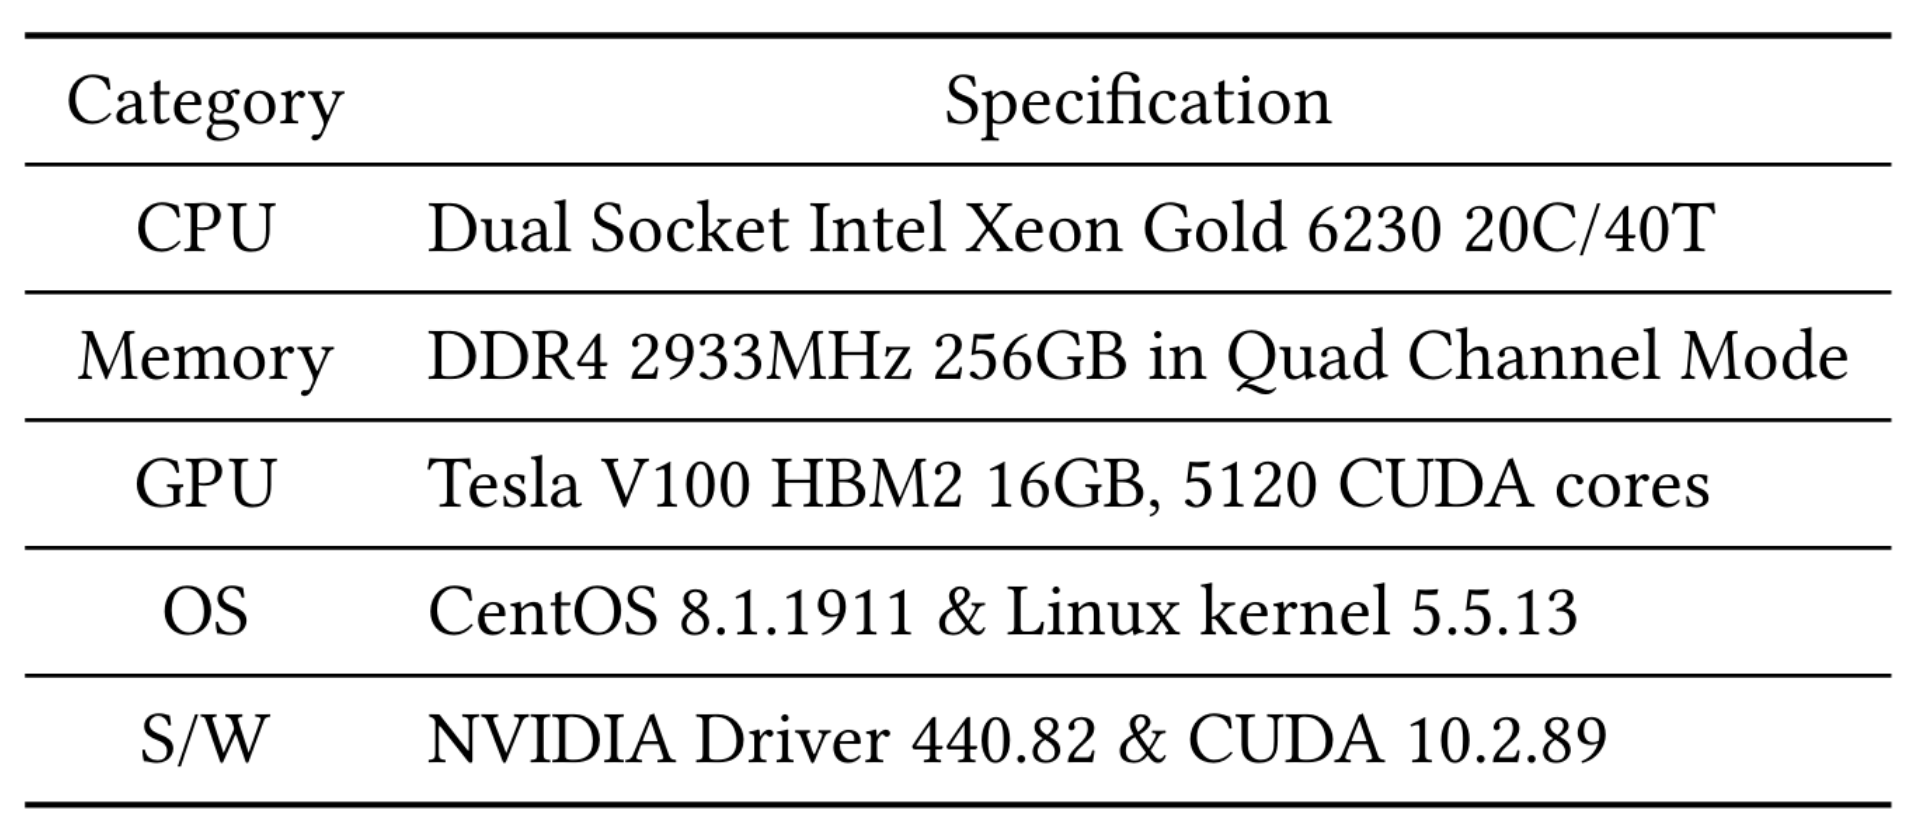
\includegraphics[width=\textwidth]{figures/system_setup.png}
            \caption{Evaluation system configuration}
        \end{figure}
    \end{minipage}\hfill
    \end{center} 
\end{frame}

\begin{frame}[fragile] \frametitle{Эксперименты: данные}
    \begin{center}
    \begin{minipage}[m]{0.95\linewidth}
        \begin{figure}
            \centering
            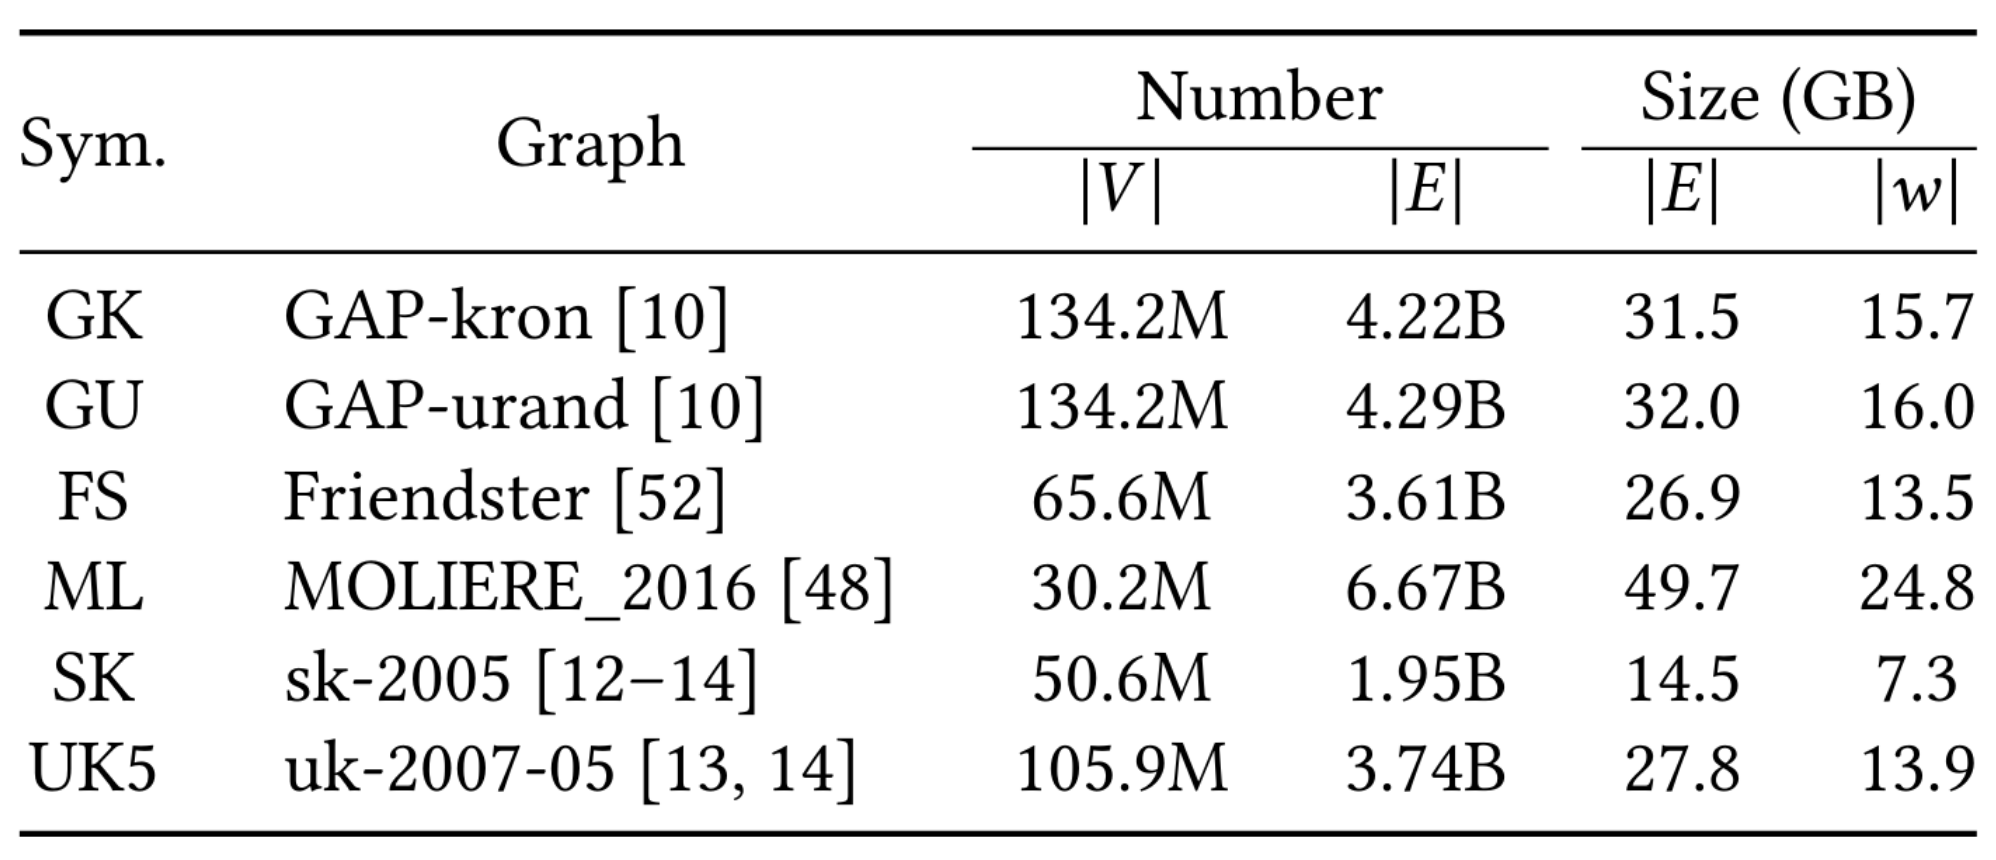
\includegraphics[width=\textwidth]{figures/datasets.png}
            \caption{Graph Datasets. $V$ = Vertex, $E$ = Edge, and $w$ = Weight}
        \end{figure}
    \end{minipage}\hfill
    \end{center} 
\end{frame}

\begin{frame}[fragile] \frametitle{Эксперименты: данные}
    \begin{itemize}
        \item Вершины и ребра индексируются 8 байтными числами
        \item Веса представляются 4 байтными числами
        \item Средняя степень вершины 38
        \item Средняя степень вершины в ML: 222
        \item Для алгоритмов с одной стартовой вершиной случайным образом выбирались 64 начальные вершины, которые имеют не 0 число исходящих ребер
    \end{itemize}
\end{frame}

\begin{frame}[fragile] \frametitle{Эксперименты: результаты}
     \begin{center}
    \begin{minipage}[m]{0.95\linewidth}
        \begin{figure}
            \centering
            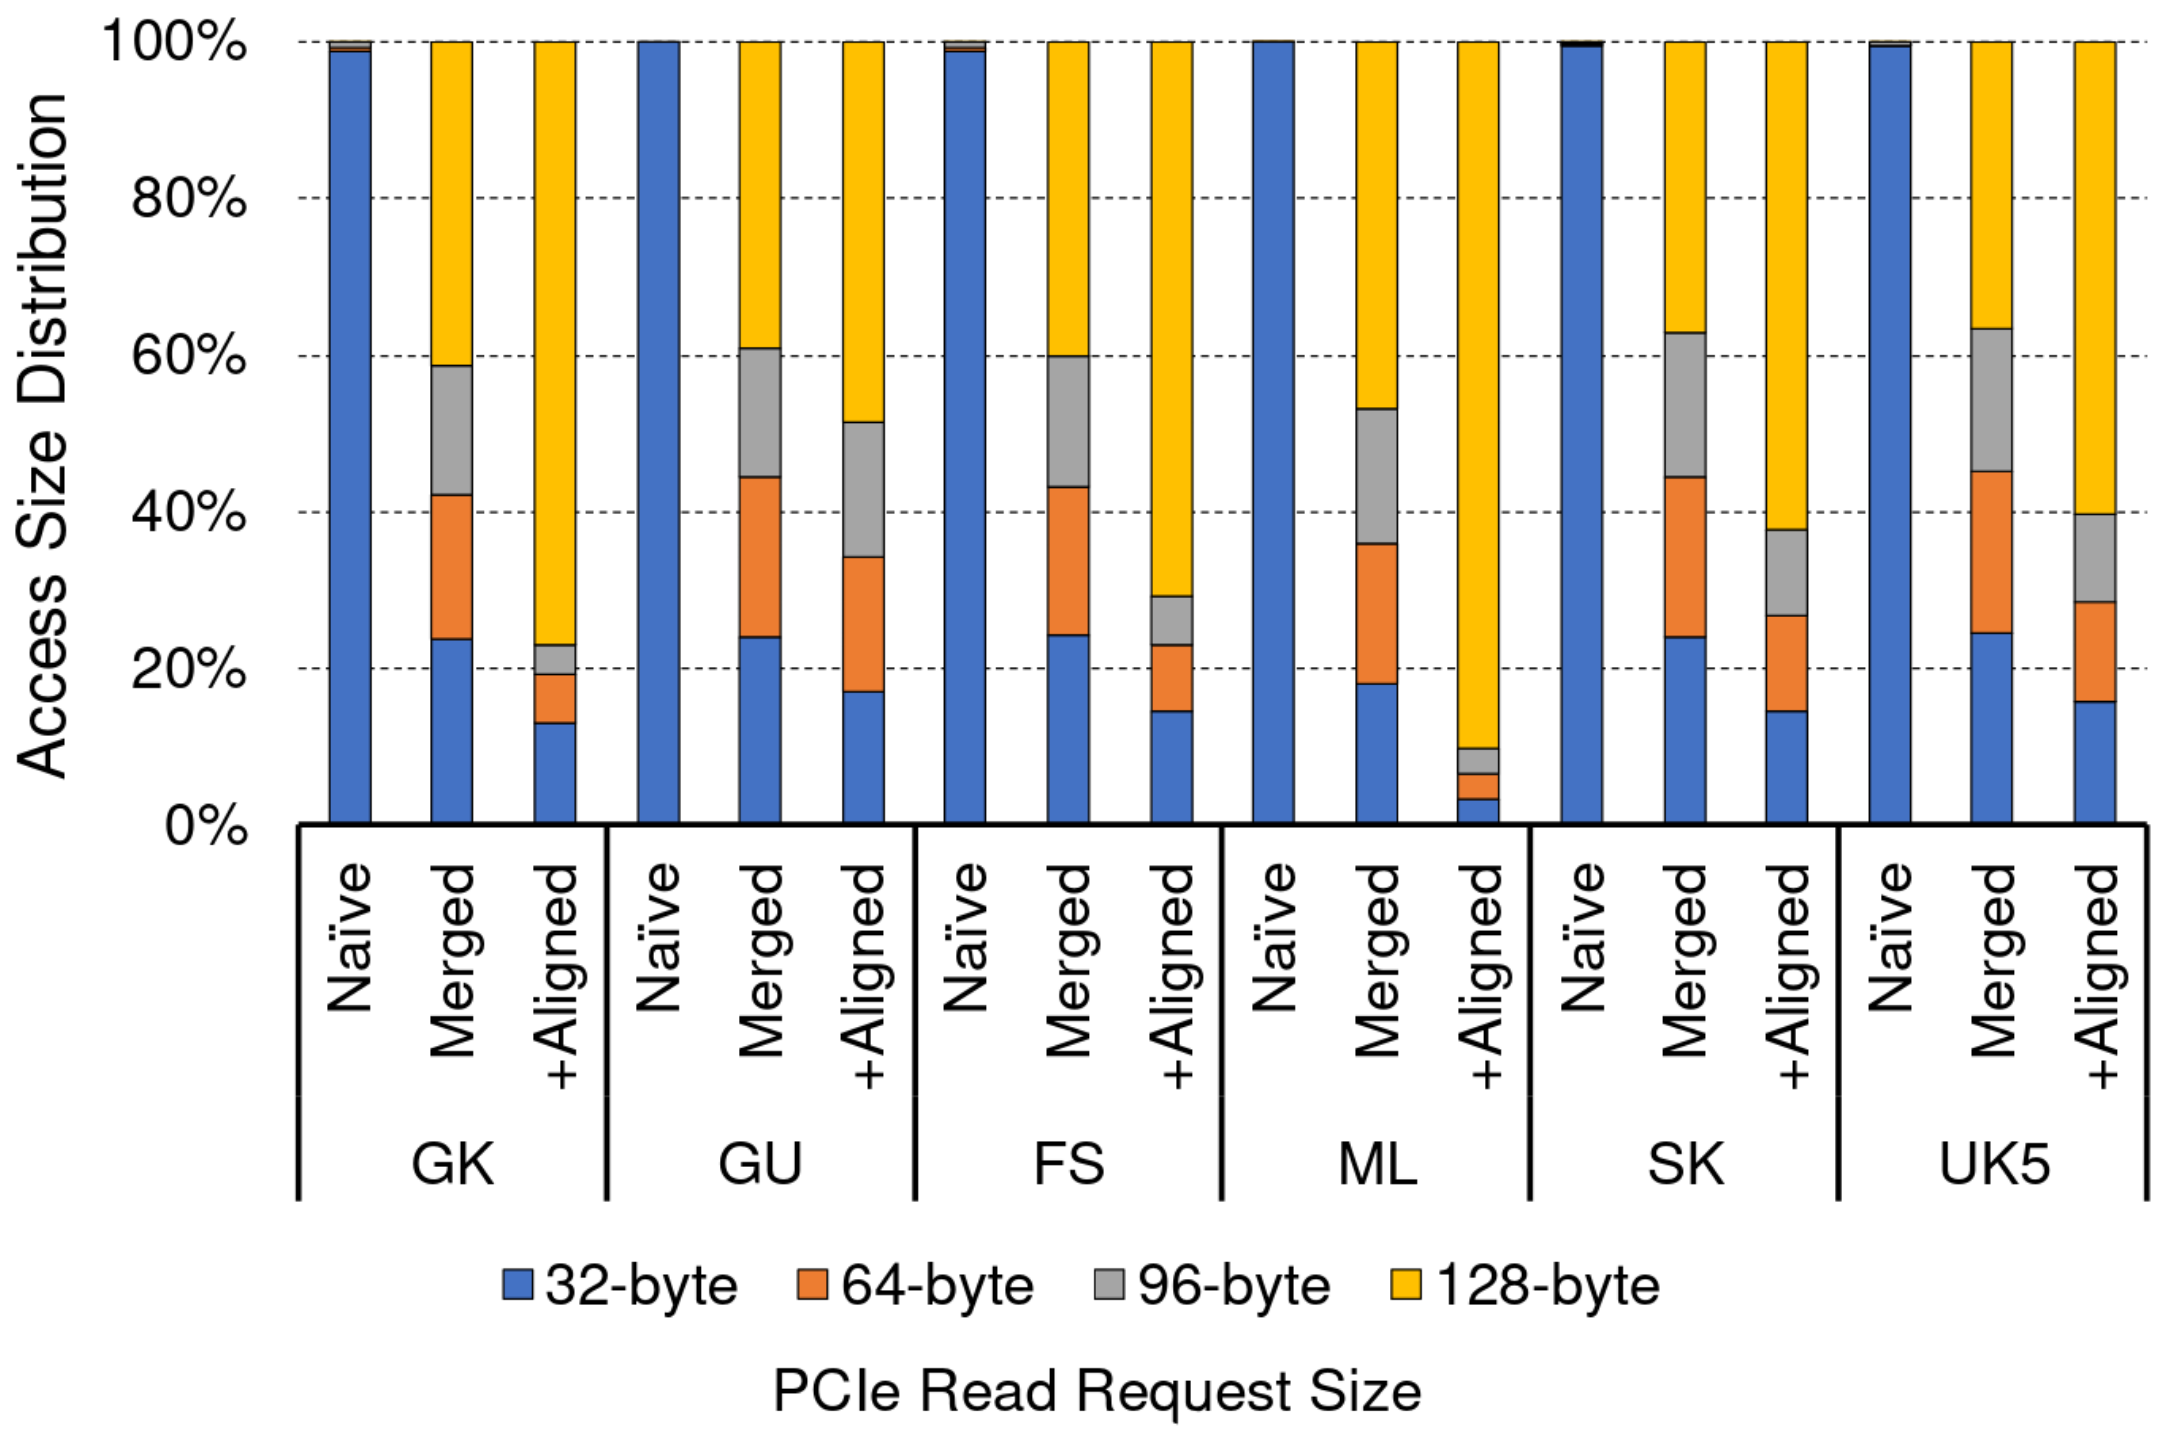
\includegraphics[width=0.7\textwidth]{figures/request_size.png}
            \caption{Distribution of PCIe read request sizes in BFS.+Aligned is abbreviation for Merged+Aligned. As the merged and aligned optimizations are added, the BFS application generates more 128-byte requests for efficient access}
        \end{figure}
    \end{minipage}\hfill
    \end{center}
\end{frame}

\begin{frame}[fragile] \frametitle{Эксперименты: результаты}
     \begin{center}
    \begin{minipage}[m]{0.95\linewidth}
        \begin{figure}
            \centering
            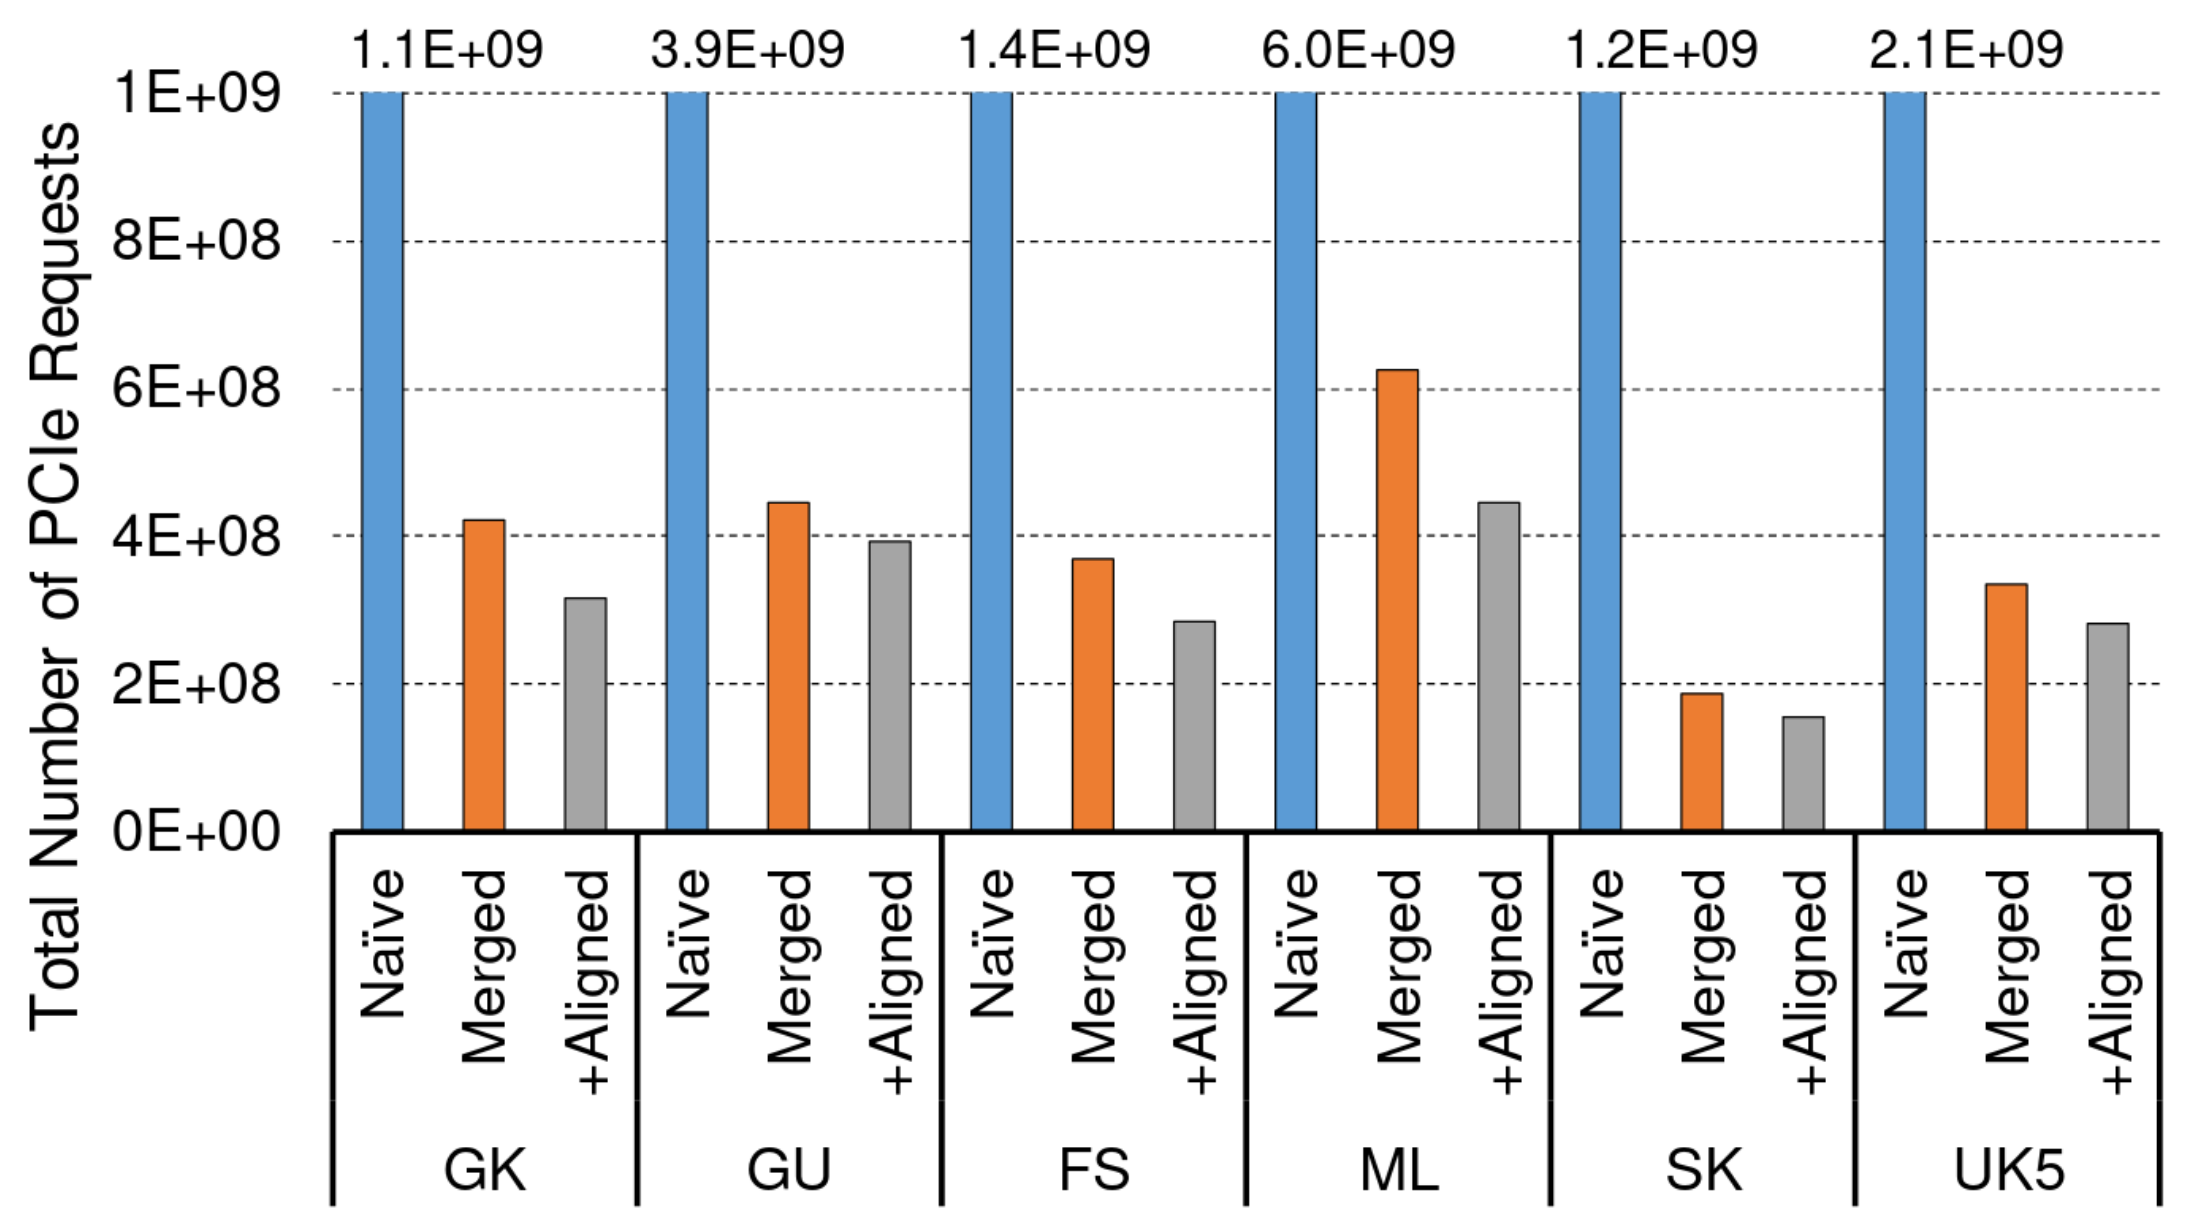
\includegraphics[width=0.7\textwidth]{figures/num_of_requests.png}
            \caption{Number of PCIe requests sent for Na\"{\i}ve, Merged and Merged+Aligned implementations while executing BFS on various graph. Collected from FPGA. Merged optimization reduces the PCIe memory requests by up to 83.3\% compared to the Na
            "{\i}ve implementation. Merged+Aligned optimization can further reduce the PCIe memory requests by up to 28.8\%. +Aligned is abbreviation for Merged+Aligned}
        \end{figure}
    \end{minipage}\hfill
    \end{center}
\end{frame}

\begin{frame}[fragile] \frametitle{Эксперименты: результаты}
     \begin{center}
    \begin{minipage}[m]{0.95\linewidth}
        \begin{figure}
            \centering
            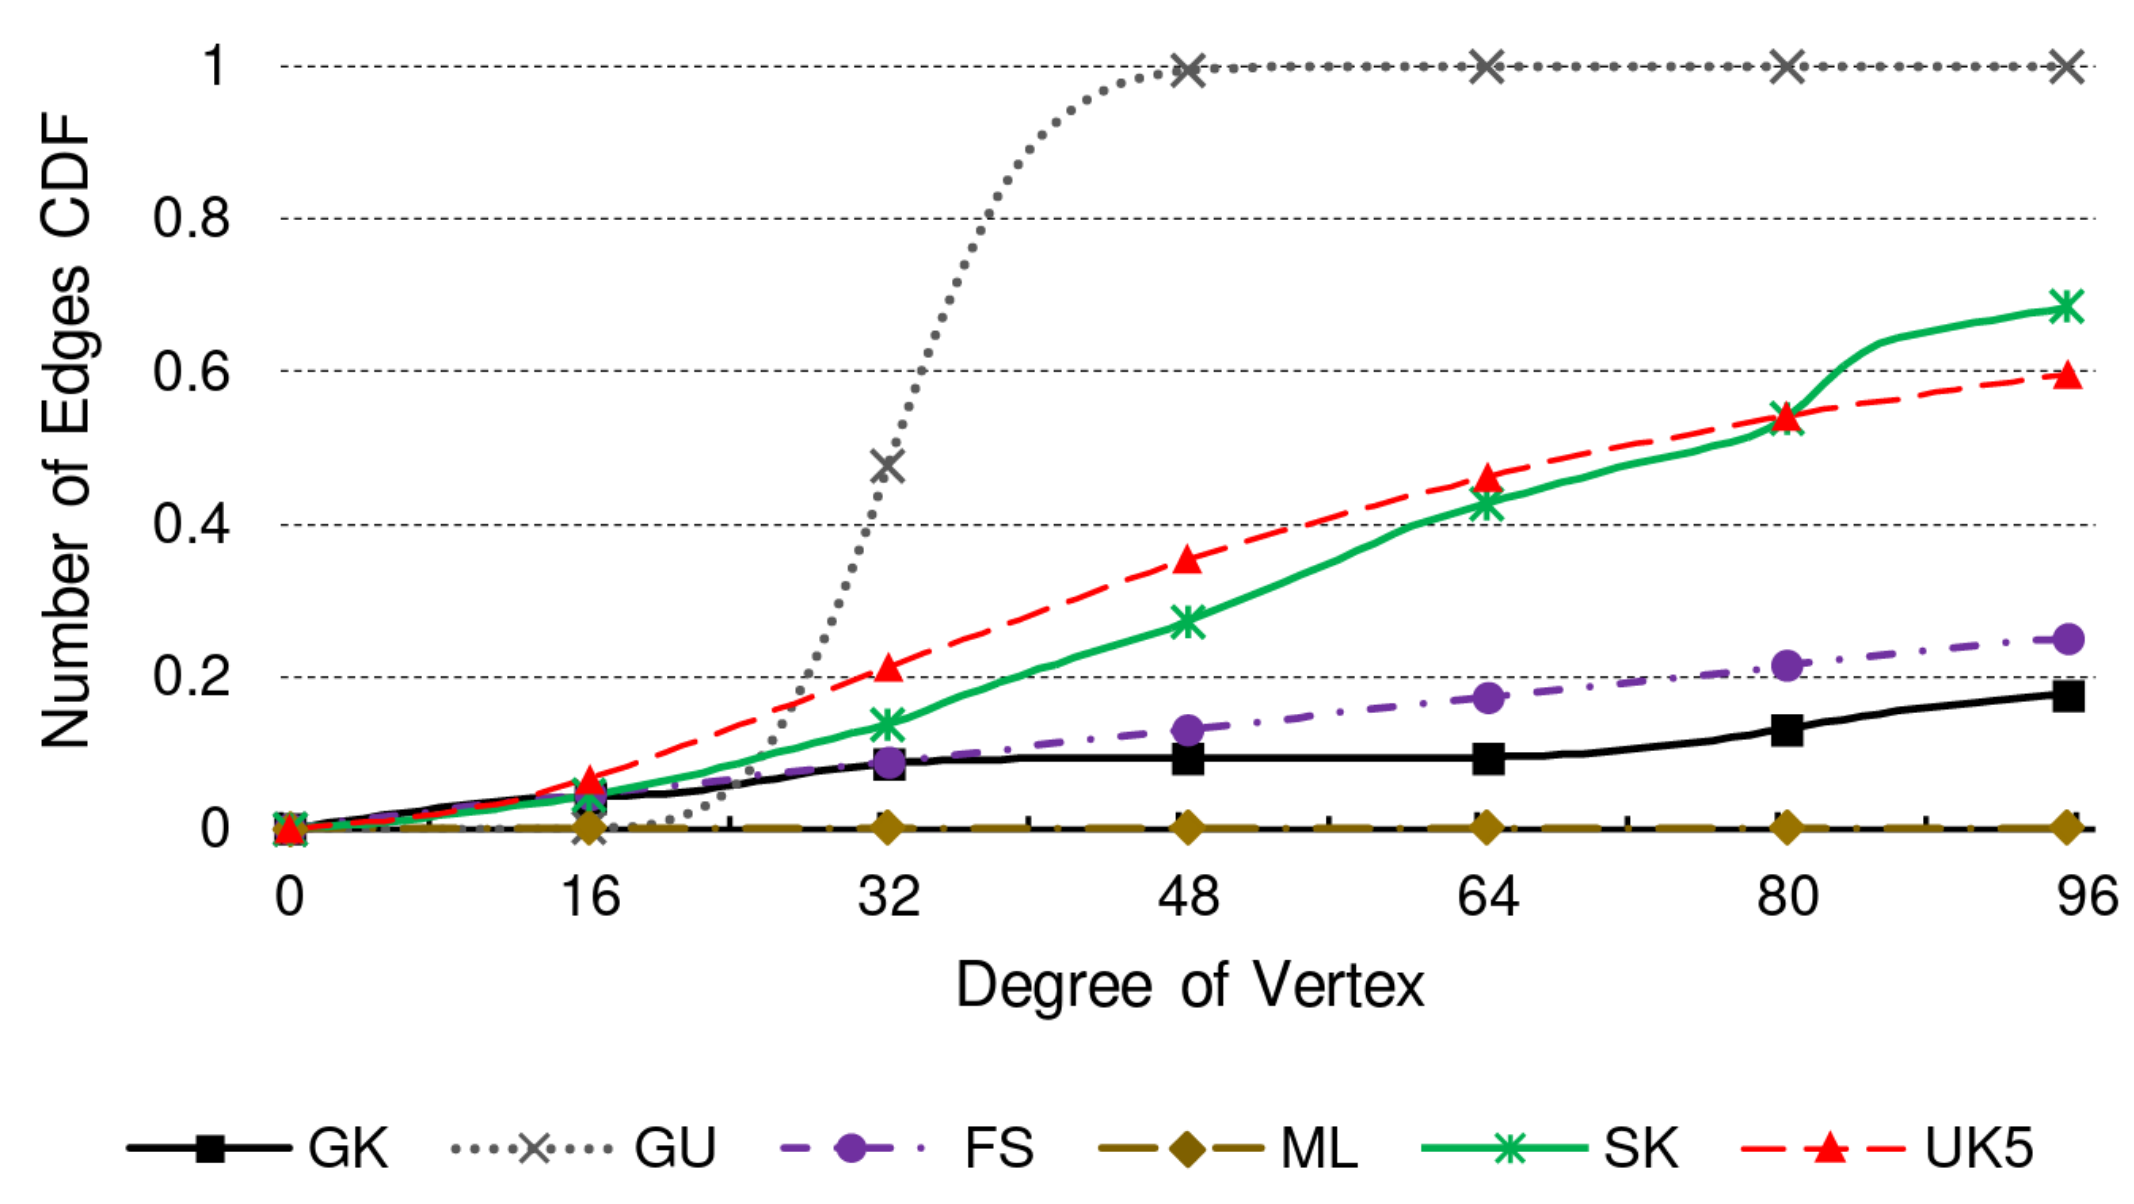
\includegraphics[width=0.7\textwidth]{figures/cdf.png}
            \caption{Number of edges CDF of evaluation graph. This plot provides us a better understanding of the distribution of the neighbor list sizes in the graphs. For example, the GU graph has all of its edges associated with vertices with degree between 16 and 48, meaning the neighbor lists contain at most 48 neighbors}
        \end{figure}
    \end{minipage}\hfill
    \end{center}
\end{frame}

\begin{frame}[fragile] \frametitle{Эксперименты: результаты}
     \begin{center}
    \begin{minipage}[m]{0.95\linewidth}
        \begin{figure}
            \centering
            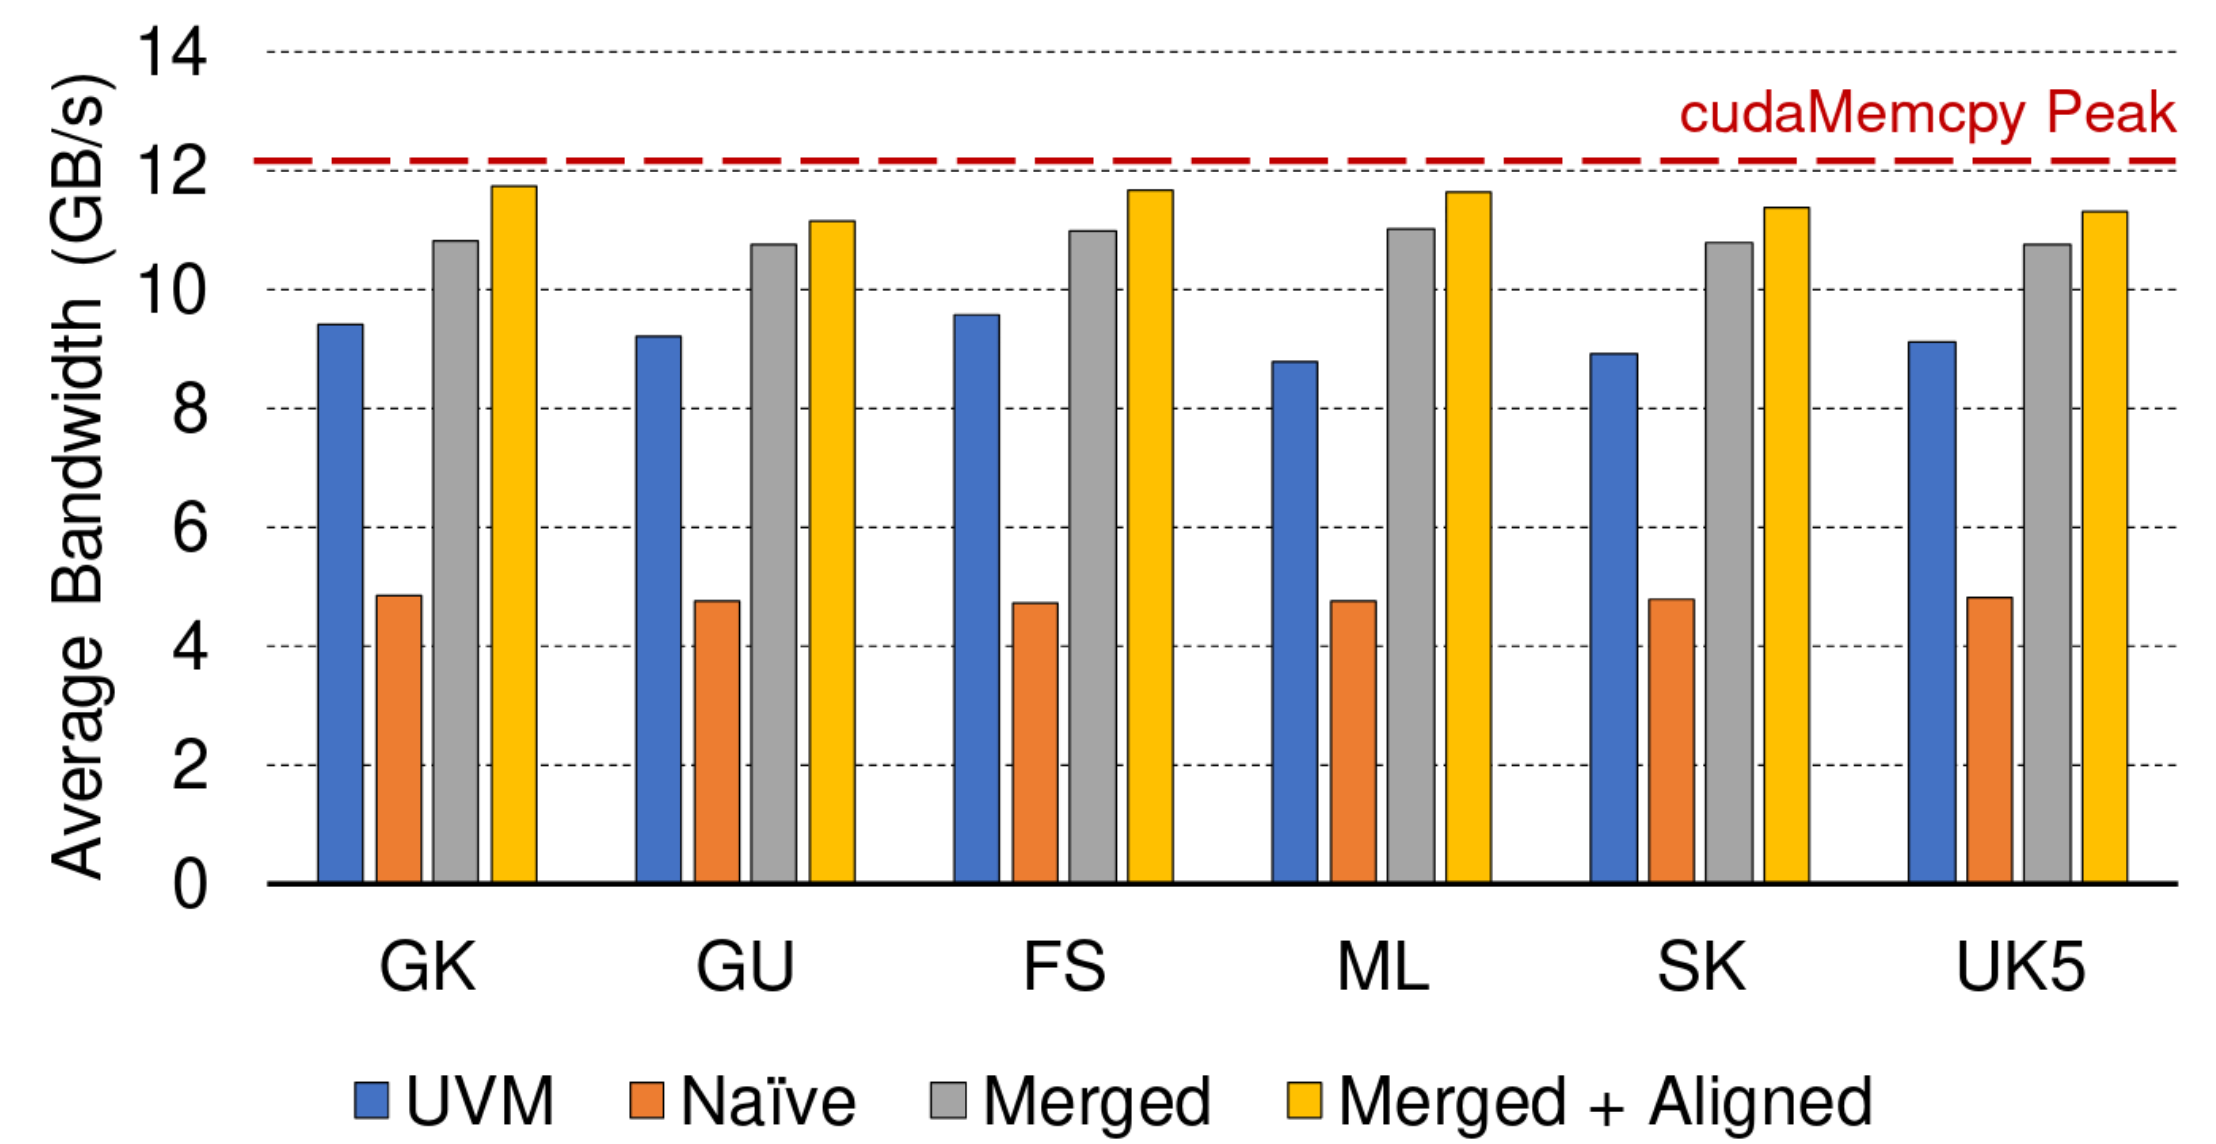
\includegraphics[width=0.8\textwidth]{figures/bandwidth.png}
            \caption{Average PCIe 3.0 x16 bandwidth utilization of the different implementations executing BFS. The Merged+Aligned implementation can nearly saturate the available PCIe bandwidth}
        \end{figure}
    \end{minipage}\hfill
    \end{center}
\end{frame}

\begin{frame}[fragile] \frametitle{Эксперименты: результаты}
     \begin{center}
    \begin{minipage}[m]{0.95\linewidth}
        \begin{figure}
            \centering
            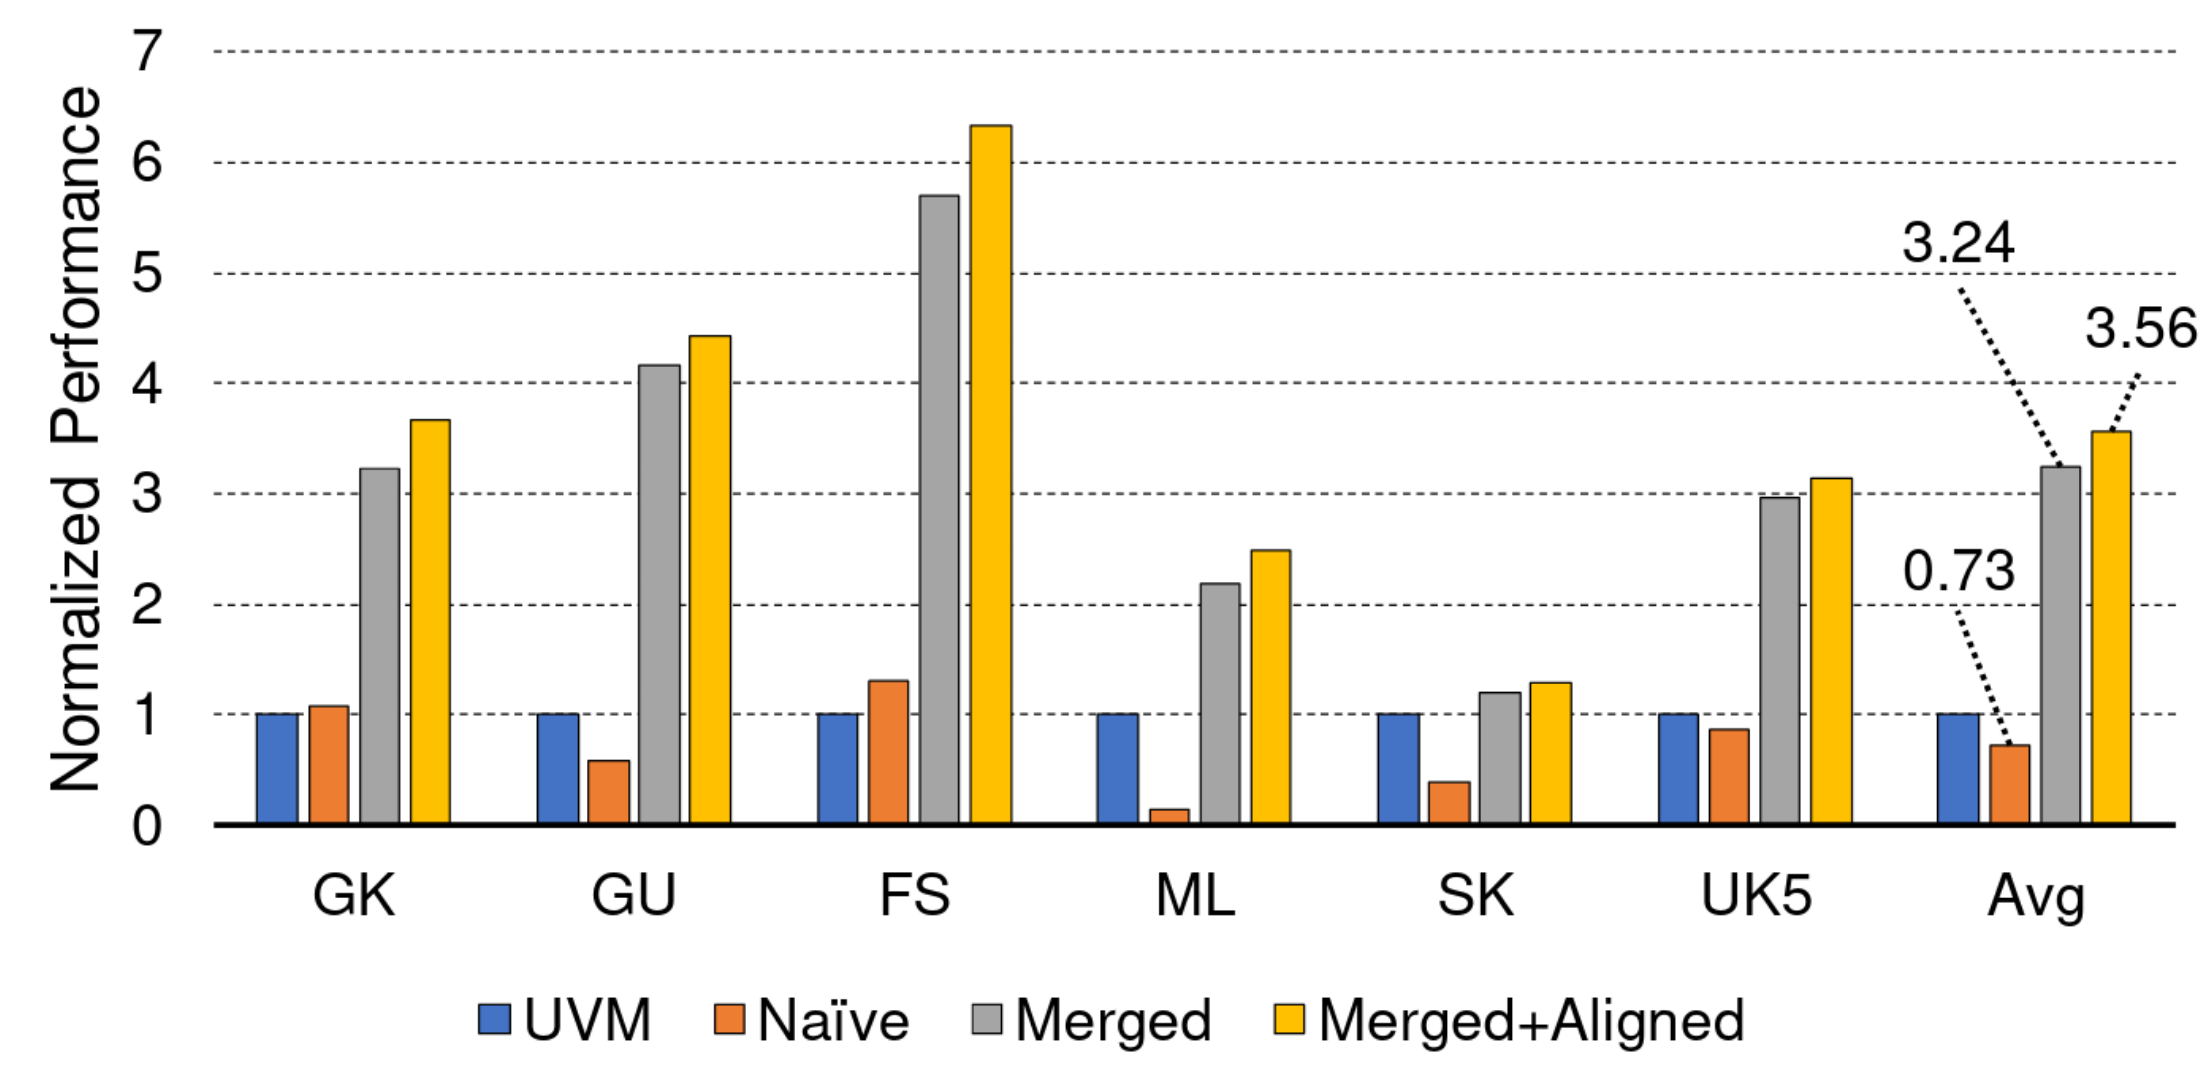
\includegraphics[width=0.8\textwidth]{figures/performance.png}
            \caption{BFS performance of the Na\"{\i}ve, Merged and Merged+Aligned implementations  against the UVM baseline. EMOGI’s Merged+Aligned implementation provides the best performance across all graphs}
        \end{figure}
    \end{minipage}\hfill
    \end{center}
\end{frame}

\begin{frame}[fragile] \frametitle{Эксперименты: результаты}
     \begin{center}
    \begin{minipage}[m]{0.95\linewidth}
        \begin{figure}
            \centering
            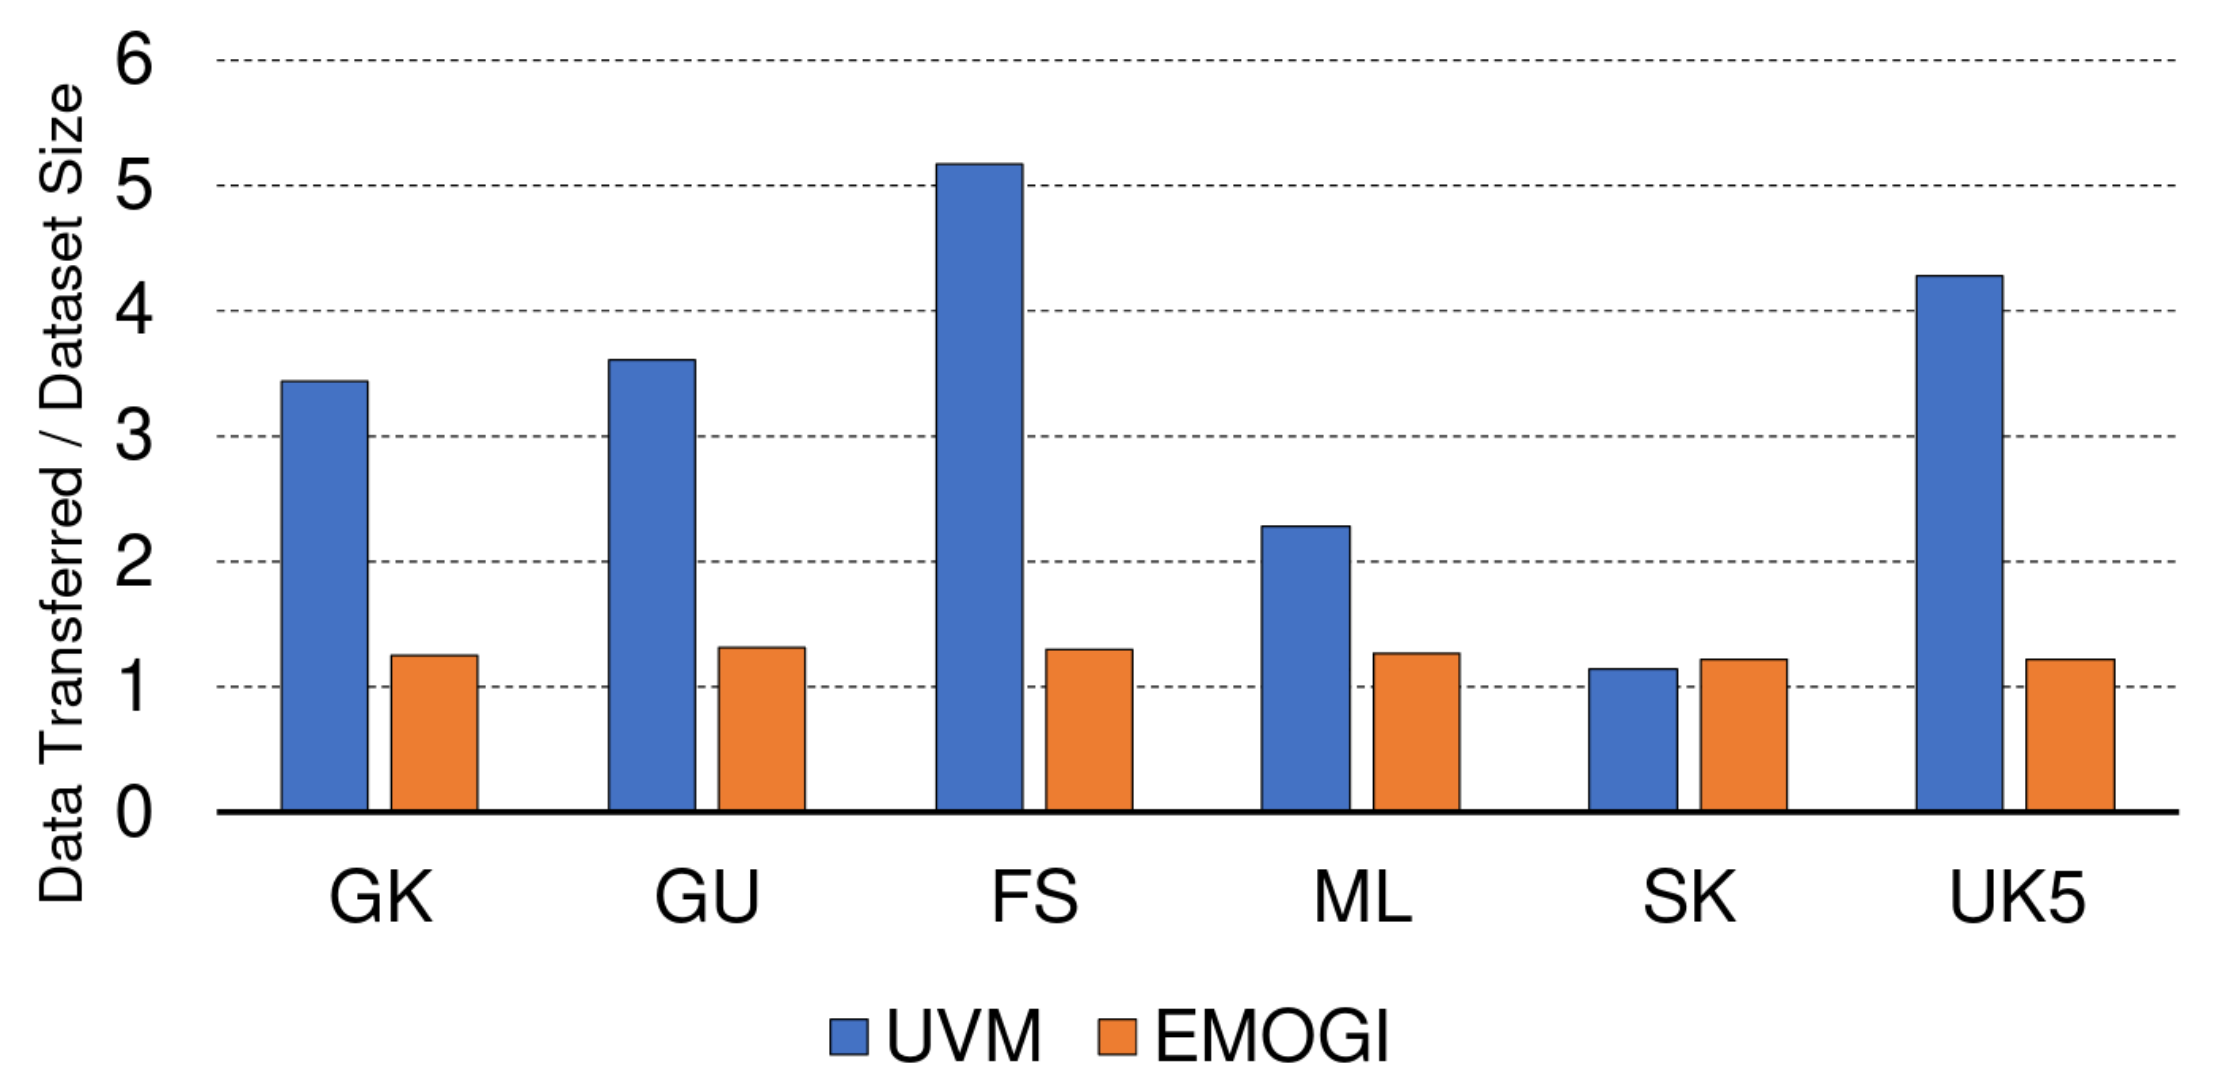
\includegraphics[width=0.8\textwidth]{figures/transfered_data.png}
            \caption{I/O Read Amplification of EMOGI and the UVM baseline while performing BFS. EMOGI has far less I/O read amplification when the graph sizes are significantly larger than the GPU memory}
        \end{figure}
    \end{minipage}\hfill
    \end{center}
\end{frame}

\begin{frame}[fragile] \frametitle{Эксперименты: результаты}
     \begin{center}
    \begin{minipage}[m]{0.95\linewidth}
        \begin{figure}
            \centering
            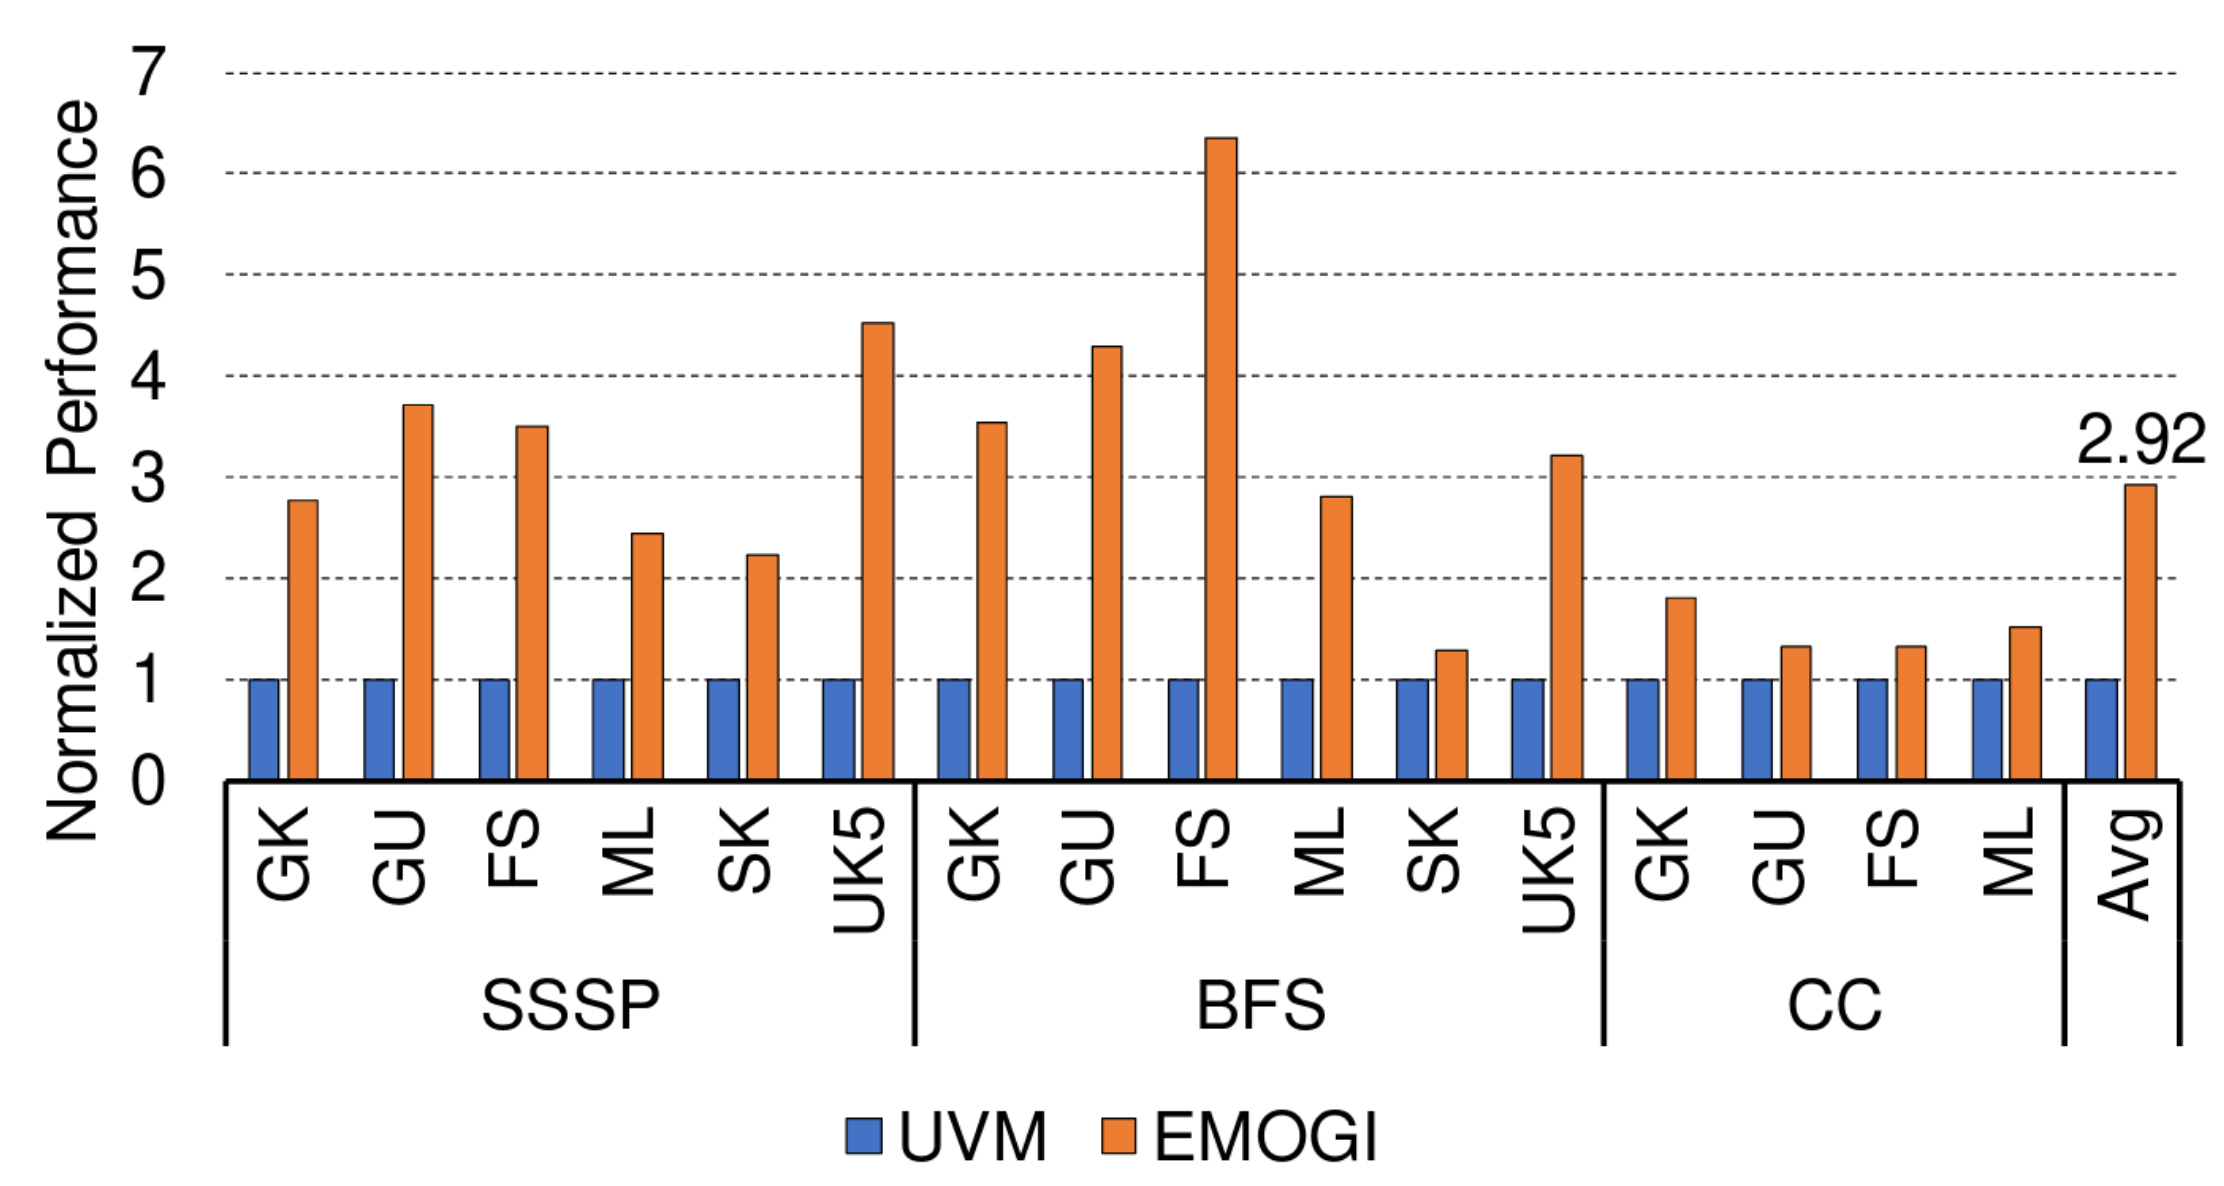
\includegraphics[width=0.8\textwidth]{figures/overall_performance.png}
            \caption{Performance comparison between UVM and EMOGI wit hdifferent graph traversal applications. EMOGI is 2.92× faster that UVM on average}
        \end{figure}
    \end{minipage}\hfill
    \end{center}
\end{frame}

\begin{frame}[fragile] \frametitle{Эксперименты: результаты}
     \begin{center}
    \begin{minipage}[m]{0.95\linewidth}
        \begin{figure}
            \centering
            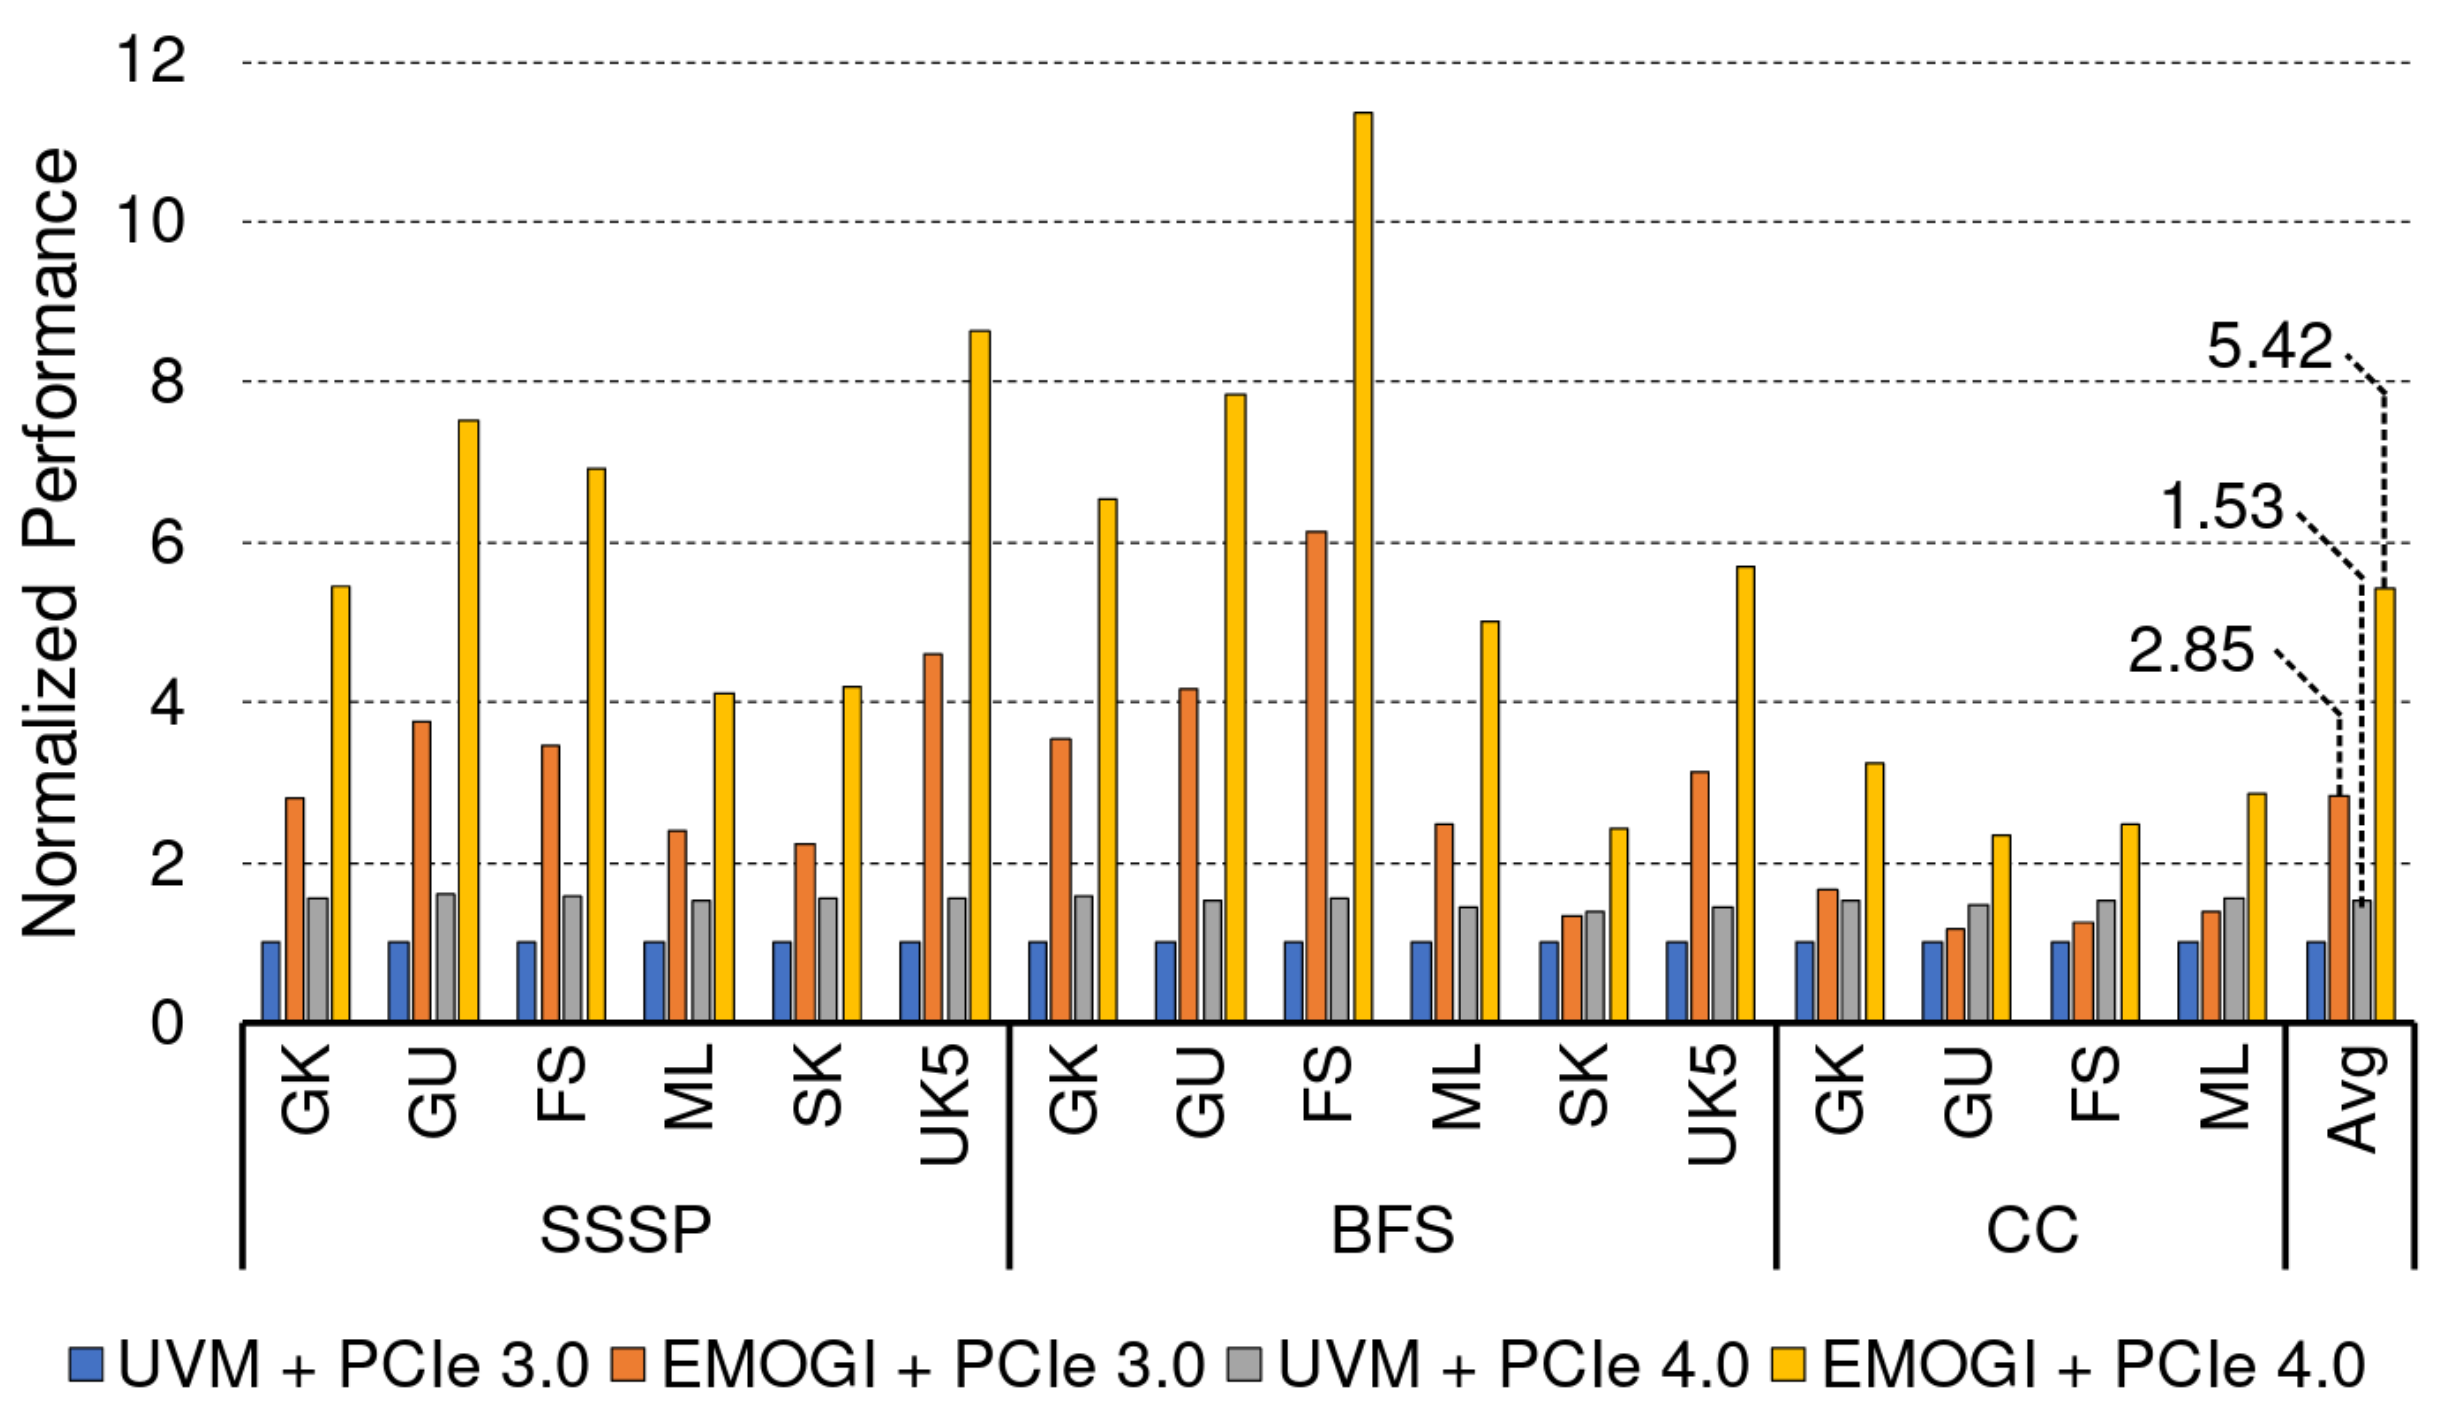
\includegraphics[width=0.8\textwidth]{figures/scalability.png}
            \caption{Performance comparison between UVM and EMOGI using PCIe 3.0 and PCIe 4.0. All results are measured in DGX A100. EMOGI is able to scale almost linearly with the PCIe bandwidth}
        \end{figure}
    \end{minipage}\hfill
    \end{center}
\end{frame}

\begin{frame} \frametitle{Дополнительно}
    \begin{itemize}
        \item Почта: \href{mailto:egororachyov@gmail.com}{egororachyov@gmail.com}
        \item Материалы презентации:
        {
            \begin{itemize}
                \item {EMOGI: Efficient Memory-access for Out-of-memory Graph-traversal In GPUs, Seung Won Min, Vikram Sharma Mailthody, Zaid Qureshi, Jinjun Xiong, Eiman Ebrahimi, Wen-mei Hwu, ссылка: 
              \href{https://arxiv.org/abs/2006.06890}{https://arxiv.org/abs/2006.06890}} 
            \end{itemize}
        }
    \end{itemize}
\end{frame}

\end{document}
